
\documentclass[11pt,a4paper]{article}

\usepackage[T1]{fontenc}
\usepackage[utf8]{inputenc} % Safe w/ pdflatex; ignored in modern engines.
\usepackage{lmodern}        % Better Latin Modern version of Computer 
\usepackage{geometry}
\geometry{margin=1in} % Change as needed.
\usepackage{microtype} % Better kerning/justification.
\usepackage{setspace}  % \onehalfspacing, etc., if reviewers want.
\usepackage{parskip}   % Turn paragraphs into skip-separated blocks 
\usepackage{listings}
\usepackage{tcolorbox}
\tcbuselibrary{listings} % Integrates tcolorbox with listings
\usepackage{xcolor}
\usepackage[authoryear]{natbib}
% Define colors and style for JSON highlighting
\definecolor{stringcolor}{rgb}{0.4,0.7,0.4}
\definecolor{numbercolor}{rgb}{0.5,0.5,1}
\definecolor{keycolor}{rgb}{0.1,0.4,0.7}

\lstdefinestyle{jsonstyle}{
    language=Java, % No default JSON language, but Java is a close match for keywords
    basicstyle=\small\ttfamily,
    morestring=[b]",
    moredelim=[il][\color{keycolor}]{-}, % for keys before colon
    stringstyle=\color{stringcolor},
    keywordstyle=\color{numbercolor},
    morekeywords={true,false,null},
    showstringspaces=false,
    breaklines=true,
    frame=none
}

% -------------------------------- Graphics & Color --------------------------
\usepackage{graphicx}
\usepackage{float} 
\usepackage{xcolor}
\usepackage{tcolorbox}
% -------------------------------- Math & Theorems --------------------------
\usepackage{amsmath,amssymb,amsthm}

% Example theorem setups (edit or remove):
\newtheorem{theorem}{Theorem}
\newtheorem{lemma}{Lemma}
\theoremstyle{remark}\newtheorem{remark}{Remark}

% -------------------------------- Tables & Units ----------------------------
\usepackage{booktabs}  % Pretty tables
\usepackage{siunitx}   % Nice number & unit formatting; optional
\sisetup{detect-all=true}

% -------------------------------- References & Links ------------------------
\usepackage{hyperref}
\hypersetup{
  colorlinks=true,
  linkcolor=blue,
  citecolor=blue,
  urlcolor=blue,
  pdfauthor={Raunak Narwal},
  pdftitle={BIGBOY1.2}
}
\usepackage[capitalize,nameinlink]{cleveref} % \cref{fig:foo}

% -------------------------------- Author Blocks -----------------------------
% Flexible multi-author formatting using authblk.
\usepackage{authblk}
% Optional ORCID icons (works best w/ PDFLaTeX if you have the package):
% \usepackage{orcidlink} % then use \orcidlink{0000-0000-0000-0000}

% -------------------------------- Title Style Toggle ------------------------
% If you want a global small-caps toggle for the *main title*, use this.
\newif\ifTitleSmallCaps
\TitleSmallCapstrue % default ON; change to ...false to disable.

% Macro that applies the toggle:
\newcommand{\TitleCase}[1]{\ifTitleSmallCaps\textsc{#1}\else#1\fi}

% Undertitle (subtitle) + header text macros. Change or leave empty.
\newcommand{\undertitle}{}
\newcommand{\headertext}{}

% Short title for running header (optional):
\newcommand{\shorttitle}{BIGBOY1.2}
\documentclass{article}
\usepackage[table]{xcolor}
\usepackage{colortbl}
\usepackage{array}
\usepackage{caption}

% Define colors
\definecolor{lightgray}{gray}{0.95}  % 5% black
\definecolor{midgray}{gray}{0.5} 
% We'll set running headers using fancyhdr.
\usepackage{fancyhdr}
\pagestyle{fancy}
\fancyhf{}
\lhead{\shorttitle}
\rhead{\headertext}
\cfoot{\thepage}
\renewcommand{\headrulewidth}{0.4pt}

% -------------------------------- Keywords Macro ----------------------------
\newcommand{\keywords}[1]{\par\vspace{0.5em}\noindent\textbf{Keywords:}~#1\par}

% -------------------------------- Abstract Env (styled) ---------------------
% A centered bold small-caps heading + quote block feel.
\renewenvironment{abstract}{%
  \vspace{1em}%
  \begin{center}\bfseries\large\scshape Abstract\end{center}%
  \begin{quote}
}{\end{quote}\vspace{1em}}

% -------------------------------- Section Spacing Tweaks --------------------
% Slightly tighter than default article.
\usepackage{titlesec}
\titlespacing*{\section}{0pt}{2.0ex plus 0.5ex minus 0.2ex}{1.0ex}
\titlespacing*{\subsection}{0pt}{1.5ex plus 0.5ex minus 0.2ex}{0.8ex}
\titlespacing*{\subsubsection}{0pt}{1.0ex plus 0.3ex minus 0.2ex}{0.5ex}

% Optional: Section font style customization.
\titleformat{\section}{\large\bfseries}{\thesection}{1ex}{}
\titleformat{\subsection}{\normalsize\bfseries}{\thesubsection}{1ex}{}
\titleformat{\subsubsection}{\normalsize\itshape}{\thesubsubsection}{1ex}{}

% -------------------------------- Bibliography ------------------------------
% Choose ONE of the two options below.

% --- Option 1 (natbib + .bib) ------------------------------------------------
% \usepackage[numbers,sort&compress]{natbib}
% \bibliographystyle{unsrtnat}

% --- Option 2 (biblatex) ----------------------------------------------------
% \usepackage[backend=biber,style=numeric,sorting=none]{biblatex}
% \addbibresource{refs.bib}

% ============================================================================
% Document Metadata ----------------------------------------------------------
% ============================================================================

% Use the \TitleCase macro if you want global small caps; otherwise remove it.
\title{\TitleCase{BIGBOY1.2: \textsc{Generating Realistic Synthetic Data for Disease Outbreak Modelling and Analytics}}}

% Example multi-author block. Replace with real info.
\author[1]{Raunak Narwal\thanks{\texttt{ms23177@iisermohali.ac.in}}}
\author[2]{Syed Abbas\thanks{\texttt{abbas@iitmandi.ac.in}, internship supervisor}}

\affil[1]{Department of Mathematics,IISER Mohali, India}
\affil[2]{Department of Mathematics, IIT Mandi, India}

% Date: leave blank for no date.
\date{\today}

% ============================================================================
% Begin Document -------------------------------------------------------------
% ============================================================================

\begin{document}

% In case you want to override smallcaps *after* metadata:
% \TitleSmallCapsfalse
% \title{BIGBOY1.2: \textsc{Synthetic Dataset Generator} for Disease Outbreak Modelling and Visualisations}
% \maketitle after toggling.

\maketitle
\tcbset{
    colback=black!5!white,  % background color (5% black = light grey)
    colframe=black!5,      % border color (50% black = dark grey)
    boxrule=0.5pt,          % border thickness
    arc=2mm,                % rounded corners
    left=5pt,right=5pt,top=5pt,bottom=5pt, % padding
    boxsep=5pt
}

\renewenvironment{abstract}{
  \begin{center}
    \bfseries\large\scshape Abstract
  \end{center}
  \begin{tcolorbox}
}{
  \end{tcolorbox}
}

\begin{abstract}
Modelling disease outbreak models remains challenging due to incomplete surveillance data, noise, and limited access to standardized datasets. We have created \textbf{BIGBOY1.2}, an open synthetic dataset generator that creates configurable epidemic time series and population-level trajectories suitable for benchmarking modelling, forecasting, and visualisation. The framework supports SEIR and SIR-like compartmental logic, custom seasonality, and noise injection to mimic real reporting artifacts. BIGBOY1.2 can produce datasets with diverse characteristics, making it suitable for comparing traditional epidemiological models (e.g., SIR, SEIR) with modern machine learning approaches (e.g., SVM, neural networks). .\par
\keywords{synthetic data; epidemiology; outbreak modelling; visual analytics; SEIR}
\end{abstract}

% --------------------------- Main Matter -------------------------------------
\section{Introduction}
Infectious diseases have repeatedly challenged the global health system, economies, and societies. During the past few decades, we have witnessed outbreaks such as SARS (2003) \citep{who_sars_2003},\citep{cdc_h1n1_2009}, Ebola \citep{who_ebola_2014}, and COVID-19 \citep{who_covid_2020}, which have demonstrated how quickly pathogens can disrupt normal life and healthcare systems, causing unprecedented economic and social consequences. In such scenarios, epimedic modelling plays significant role in disease outbreak prediction, policymaking and timely intervention stratergies \citep{keeling_rohani_2011}. But epidemiological modelling remains heavily dependent on the availability and quality of outbreak data. Missing dates, reporting delays and substandard datasets make it challenging to train and benchmark models. That has led to our increased interest in synthethic data generation, BIGBOY1.2 could generate reality mimicking datasets and visualtions which make them ideal for benchmarking models, stress testing algorithms, and conducting reproducible experiments \citep{goncalves_synthetic_2020}.
\subsection{Background}
Accurate modeling and forecasting of disease outbreaks have been a crucial topic for public health planning and decision making. Classical epidemiological models, such as compartmental models (SIR, SEIR) have proven their effectiveness for understanding transmission dynamics. These can be used to estimate parameters like basic reproduction number $R_0$, beta effective and estimate interventions. However these models are idealistic and generally different from real world data. Real world data is noisy, incomplete and subject to irregular reporting due to many factors such as delays in case confirmation, underreporting and inconsistent testing policies across different regions. \\
The COVID-19 pandemic further highlighted the need for high quality datasets for epidemic modelling. Most studies relied on the use of fragmented and incomplete datasets, which limited the reliability of forecasts and their ability to reproduce. Data inconsistencies such as negative incidence values (due to backlogs and correction) created major challengers for data-driven machine learning models, that require large, well structured datasets. As a result, forecasting methods on real world datsets is often inconclusive. \\
To limitations have compelled researcherrs to use synthethic data. Our synthethic data generator , BIGBOY1.2 allows for complete control over epidemic parameters, which includes population, layers, seasonality, interventions and stochastic variations. It provides an invaluable testbed for benchmarking forecasting models under controlled scenarios, enabling rigorous evaluation of algorithmic performance in condition where real world data would be insufficient or biased. But most existing synthethic dataset tools are either very simplistic and fail to mimic the complex nature of real world outbreaks or too specialized, designed for specific disease and narrow research goals.
\subsection{Motivation for BIGBOY1.2}
As discussed before, synthethic data generators fall short in key aspects of realism, flexibilty and usability. Important factors like seasonal variation, stochastic effects and reporting biases are ignored and are tightly coupled to specific diseases or parameters settings. As a consequence, researchers resort to creating ad-hoc datasets, which lack standardization, making it difficult to compare forecasting models across studies. \\
Moreover current tools rarely integrate visual analytics with the data generation pipeline. The ability to intuitively visualize compartmental dynamics, intervention impacts is very crucial for communicating findings effectively. Without built in visualization support, the user relies on external scripts and tools, increasing complexity to even perform a basic exploratory analyses. \\
We have proposed BIGBOY1.2 , a versatile and fully configurable synthethic dataset generator for disease outbreak modeling and analytics. BIGBOY1.2 allows users to simulate epidemics with customizable transmission parameters and intervention stratergies. It also generates visual plots such as time series plots, heatmaps, phase diagrams along with datasets. BIGBOY1.2 is lightweight and easy to use, unlike many heavy ML based dataset generators. By standardizing synthethic dataset creation, BIGBOY1.2 aims to improve reproducibility and enable fair benchmarking of disease outbreak modeling.
\section{Methods}
BIGBOY1.2 is a stochastic epidemic dataset and visual plot generator which builds upon BIGBOY1. With further refinements , it presents better and more realistic datasets.
\subsection{Framework}
BIGBOY1.2 is designed to simulate realistic infectious disease outbreaks with a high degree of configurability and realism. At its core, it is build on the SEIR (Susceptible, Exposed, Infectious, Recovered) model, extended with dynamic parameters, seasonal influences, vaccination and multi wave outbreak structures. It is a multi layered and age structured SEIR model which includes a noise and reporting module to simulate real world data irregularities. Unlike traditional simulations, BIGBOY1.2 produces data that closely resembles real world epidemic curves, and also retains full control over the underlying "ground truth" parameters. This allows researchers to test forecasting methods under controlled conditions. \\
the framework is modular in design, it consists of four key layers: Parameter Initialization, where user can manually define epidemiological and behavioral parameters; Simulation Engine, integrates the SEIR based equations and accounts for time varying transmission dynamics, interventions and stochastic effects; Noise and Reporting Layers, injects realistic data artifacts like under reporting, reporting delays and random fluctuations to mimic real world surveillance data and the last layer is Output and Visualizations, which exports the datasets in csv formats, parameters in JSON format and generates a range of visual graphs from simple time series plots to advanced 3D plots. \\
BIGBOY1.2 supports three operational modes through CLI : random mode (parameters taken from predefined ranges), interactive mode (user-driven configuration), and batch mode (generates many simulations at once). The user could also use various commands from the CLI like --plots all , --population X.\\

\begin{figure}[H] 
    \centering
    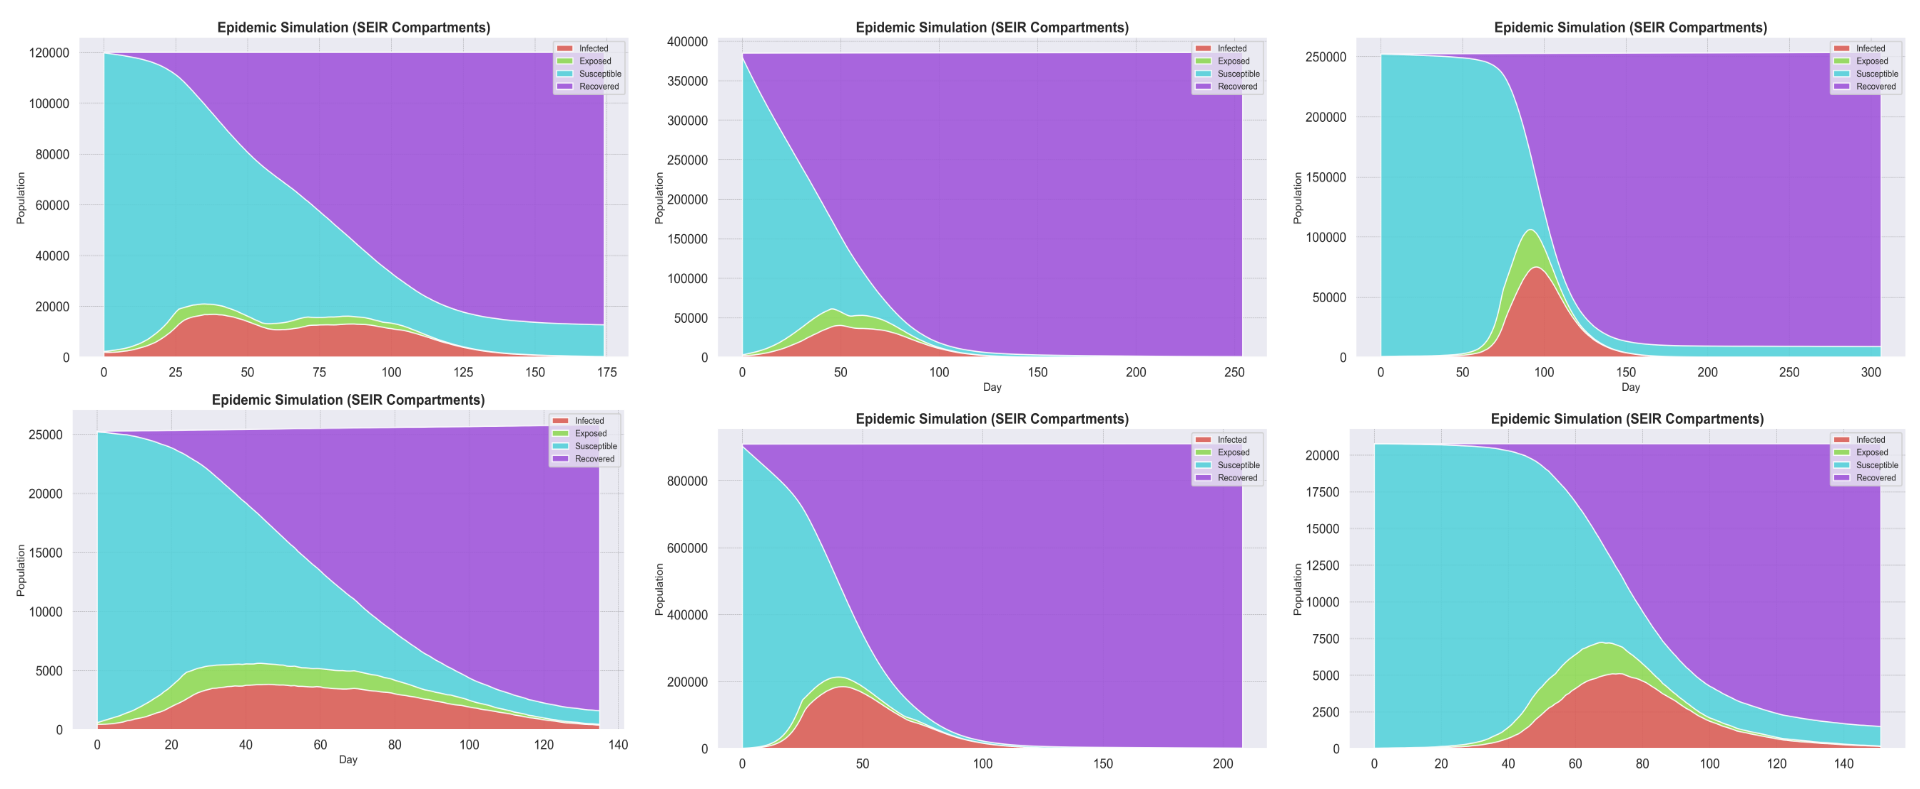
\includegraphics[width=0.8\linewidth]{SEIR_batch.png} 
    \caption{Batch mode (Python BIGBOY1.2.py batch 6 --plots all)}
    \label{fig:my_figure}
\end{figure}
\subsection{Mathematical Foundations of BIGBOY1.2}
As discussed BIGBOY1.2 builds upon the foundational SEIR model, which categorizes the population into four compartments. At any point in time, each individual belongs to one of these compartments and transition between them is governed by a set of differential equations, this has been done to incorporate real world effects such as vaccination, behavioral factors and seasonality. \\
\begin{equation} \label{eq:SEIR Fundamental}
\begin{aligned}
    \frac{dS}{dt} &= -\beta(t) \cdot \frac{SI}{N} - \nu S \\
    \frac{dE}{dt} &= \beta(t) \cdot \frac{SI}{N} - \sigma E \\
    \frac{dI}{dt} &= \sigma E - \gamma I \\
    \frac{dR}{dt} &= \gamma I + \nu S
\end{aligned}
\end{equation}

Here is a description of the model's parameters:
\begin{itemize}
    \item $S(t)$, $E(t)$, $I(t)$, and $R(t)$ represent the number of susceptible, exposed, infectious, and recovered individuals at time $t$, respectively.
    \item $N$ is the total population size (assumed constant).
    \item $\beta(t)$ is the time-varying transmission rate, which is crucial for defining how fast susceptible individuals become exposed.
    \item $\sigma$ is the rate at which exposed individuals become infectious ( the inverse of the incubation period).
    \item $\gamma$ is the recovery rate.
    \item $\nu$ is the vaccination rate, which transfers susceptible individuals directly into the recovered class.
\end{itemize}
This extended form of SEIR formulation allows BIGBOY1.2 to simulate epidemic dynamics with the effects of public health interventions such as mass vaccination. \\
Time dependent transmission rate $\beta(t)$ is a powerful and novel feature of BIGBOY1.2. The framework does not assume a constant rate of disease transmission, rather it models $\beta(t)$ as a function of multiple interacting factors, each of which represents a real world influence on transmission dynamics. 
\begin{equation} \label{eq:beta_t_definition}
\beta(t) = \beta_0 \cdot (1 - \theta_m m(t)) \cdot (1 + \theta_c c(t)) \cdot \left[ 1 + \alpha \sin\left(\frac{2\pi t}{T_s}\right) \right] \cdot \Phi(t)
\end{equation}
Where 
\begin{itemize}
    \item $\beta_0$ is the baseline transmission rate, in the absence of external modifiers.
    \item $m(t)$ is the mask adherence score at time $t$, normalized between 0 and 1.Higher the mask adherence score, higher the compliance with mask wearing. The weight $\theta_m$ controls how strongly this factor suppresses transmission.
    \item $c(t)$ is the crowdedness score, also on a normalized scale. In this, the average density of human interaction is captured, with $\theta_c$ amplifying its effect on transmission.
    \item The sinusoidal term $\alpha \sin\left( \frac{2 \pi t}{T_s} \right)$ models seasonality, it represents periodic increases or decreases in transmission due to environmental and behavioral cycles). $T_s$ is the seasonal cycle period (typically 365 days).
    \item Finally, $\Phi(t)$ is a multi-wave adjustment factor, this allows the simulation to include multiple waves ( due to new variants or changes in social behavior). It is defined as:
\end{itemize}
\begin{equation} \label{eq:phi_t}
\Phi(t) = 1 + \sum_{j=1}^{W} (\phi_j - 1) \cdot \sigma_j(t)
\end{equation}
Here each $\phi_j$ represents the peak multiplier of the $j$-th wave, and $\sigma_j(t)$ is a logistic ramp function that smoothly increases and decreases during the wave period. This component enables multiple waves having sharp rises and slow declines in transmission, a feature often seen in real epidemic data. \\
BIGBOY1.2 supports simulations with heterogeneous population structures, segmented by age and contact environments. This structure is implemented using an age and layer straified SEIR model. In confiugrations like this, the population is divided into\textit{ L }contact layers, such as household, workplace, school or community. \textit{A} age groups, such as children, adults and the elders. For each combination the simulation tracks : 
$S_{l,a}$, $E_{l,a}$, $I_{l,a}$, and $R_{l,a}$. \\
Where, \textit{l} = 1,2,...,\textit{L} denotes the contact layer and \textit{a} = 1,2,...,\textit{A} denotes the age group. \\
The force of infection $\lambda_{l,a}(t)$, or the probability per unit time that a susceptible individual in group $(l,a)$ becomes exposed, is calculated using summated contributions from all other groups based on this structured contact matrix:
\begin{equation} \label{eq:force_of_infection}
\lambda_{l,a}(t) = \sum_{l'=1}^{L} \sum_{a'=1}^{A} \beta_{l,a,l',a'}(t) \cdot \frac{I_{l',a'}(t)}{N_{l',a'}}
\end{equation}
This implies that the exposure risk for a school going kid within the community layer depends on how many infectious individuals exist in other age groups and settings, modulated by the contact matrix $C_{l,l'}$. This method brings realism into the simulation, and modeling of targeted interventions could also be enabled (like school closure or age prioritized vaccination). \\
The base SEIR model along with above extensions we have done, the BIGBOY1.2 provides a mechanistic ground truth view of an outbreak but real world surveillance data is noisy and subject to various distortions as well. To mimic this effect, BIGBOY1.2 introduces a post processing layer that applies multiple forms fo noise and uncertainity to the generated data. \\
\textbf{Travel Noise} in real epidemics, the geographical boundaries of a population is not sealed. People travel in and out of region for work, migration and emergencies. The local outbreak curves is affected by this movement, often introducing sudden spikes or dips. We have simulated this behavior through a travel noise generator, which adds or subtracts random infectious cases from the SEIR-generated curve. At each timestep $t$, the infectious compartment $I(t)$ is changed by:
\begin{equation*}
I'(t) = I(t) + \Delta_{\text{travel}}(t)
\end{equation*}
Where $\Delta_{\text{travel}}(t) \sim \mathcal{N}(\mu, \sigma^2)$, a Gaussian-distributed noise term with mean $\mu$ and standard deviation $\sigma$. These parameters can also be fixed by the user. This gives noisy, jagged , heavy tailed curves that retains the overall trend of the outbreak and also includes short term fluctuations mimicking travel between cities. \\
\textbf{Random Dropper} , another realism challenge in epidemiology is underreporting of cases, all infections are not captured. This may be due to various reasons, maybe because a computer simulation is not really a real life oubtreak scenario. So, to reflect this we have included a random dropper, that hides a certain fraction of cases from the output. 
\begin{equation*}
\text{Reported}_I(t) \sim \text{Binomial}(I'(t), p_r)
\end{equation*}
Where:
\begin{itemize}
    \item $I'(t)$ is the noisy infectious count after travel adjustment.
    \item $p_r \in [0,1]$ is the reporting probability.
\end{itemize}
This same method can be applied to independent exposed, recovered, depending on the use case.\\
We can define the output of BIGBOY1.2 as a function : 
\begin{center} % This environment centers the entire box on the page
\tcbox[
    colback=yellow!5,  % Sets the background fill to 5% black (light gray)
    colframe=black!50, % Sets the border color to 5% black
    boxrule=0.5pt,    % Defines the thickness of the border line
    arc=0mm,          % Makes the corners sharp (not rounded)
    boxsep=5pt        % Adds a little padding around the equation
]
{% The equation goes inside the argument braces of the \tcbox command
$
\mathcal{D}_{\text{BIGBOY1.2}} = \mathcal{R}\left(\mathcal{N}\left(\mathcal{S}_{\text{SEIR}}\left(\mathbf{\Theta}, \beta(t), \Phi(t), \nu, \mathbf{C}, \mathbf{M}, \mathbf{A}\right)\right)\right)
$
}
\end{center}
Where: 
\begin{itemize}
    \item $\mathcal{D}_{\text{BIGBOY1.2}}$: Final reported dataset
    \item $\mathcal{S}_{\text{SEIR}}$:  SEIR simulator that generates compartment curves over time.
    \item $\boldsymbol{\Theta}$: Core epidemiological parameters  $\{\beta_0, \gamma, \sigma, N\}$.
    \item $\beta(t)$: Time varying transmission function.
    \item $\Phi(t)$: Multi wave logistic ramp (captures new waves).
    \item $\nu$: Vaccination rate.
    \item $\mathbf{C}$: Contact matrix.
    \item $\mathbf{M}, \mathbf{A}$: Layer $\mathbf{M}$ and age-group $\mathbf{A}$ structures.
\end{itemize}

Then:
\begin{itemize}
    \item $\mathcal{N}(\cdot)$: Noise layer, which applies:
    \begin{itemize}
        \item Travel noise: $\Delta_{\text{travel}}(t) \sim \mathcal{N}(\mu, \sigma^2)$.
        \item Reporting delay.
        \item Weekend or weekday bias.
    \end{itemize}
    \item $\mathcal{R}(\cdot)$: Reporting layer, which applies:
    \begin{itemize}
        \item Random dropper: $\text{Binomial}(I'(t), p_r)$.
        \item Reporting frequency control (daily, weekly, etc.).
    \end{itemize}
\end{itemize}
The final synthetic dataset $\mathcal{D}_{\text{BIGBOY1.2}}$ is created by first running a SEIR simulation $\mathcal{S}_{\text{SEIR}}$. Then, stochastic noise $\mathcal{N}$ and distortions are injected. Finally, a reporting filter $\mathcal{R}$ simulates real-world underreporting.
\section{Simulation Pipeline}
BIGBOY1.2 is made as modular simulation engine , it is structured into well defined functional blocks. Each module processes data through a deterministic or stochastic transformation, allowing control and reproducibility. The system is configured using parameters.json and put together using python driver script. \\
\textbf{Configuration Parsing and Preprocessing} : At runtine, the simulation parses a structured paramter file that containing : 
\begin{center}
\begin{tcblisting}{
  listing only,
  hbox,
  colback=blue!5,
  colframe=black!50,
  boxrule=0.5pt,
  arc=0mm,
  boxsep=5pt,
  listing options={style=jsonstyle}
}
{
    "population": 20785,
    "days": 152,
    "initial_infected": 32,
    "mask_score": 10,
    "crowdedness_score": 7,
    "quarantine_enabled": "y",
    "seasonality_enabled": "y",
    "interventions_enabled": "n",
    "reporting_prob_min": 0.52,
    "reporting_prob_max": 0.72,
    "multi_wave": "n",
    "random_seed": 845114,
    "vaccination_enabled": "n",
    "daily_vaccination_rate": 0.016,
    "incubation_period": 5,
    "waves": [
        {
            "day": 60,
            "beta": 2.5,
            "seed": 100
        }
    ],
    "testing_rate": "medium",
    "mask_decay_rate": 0.0156,
    "travel_enabled": "n",
    "travel_max": 0,
    "mode": "random",
    "layers": 2,
    "age_groups": 3
}
\end{tcblisting}
\end{center}
Above is a sample params.json taken from a generated batch. The parser validates all input types, auto generates required times eries and prepares input buffers for the simulation. \\
\textbf{Compartmental Simulation Layer}: This module numerically integrates a layered, age structered SEIR system. It implements forward Euler integration over discrete time stamps, contains $L \times A$ compartment states in 4D tensors
\begin{center}
\tcbox[
  colback=blue!5,
  colframe=black!50,
  boxrule=0.5pt,
  arc=0mm,
  boxsep=5pt
]{% The content goes in the braces
  $S[L, A], \quad E[L, A], \quad I[L, A], \quad R[L, A]$
}
\end{center}
Transmission rate $\beta_t$ is calculated per time stamp by combining time dependent behavioral scores (mask , crowd), seasonal effects (sinusiodal) and wave ramp function. Cumulative states are kept in the memory and this engine supports toggling between homogenenous and stratified contact modes.\\
\textbf{Multiwave Modulation}, this submodule applies wave shpaed multipliers on beta effective. \textbf{Noise Injection Module}, wraps the raw SEIR outputs and introduces realistic distortions such as tavel noise, delay, radnom modulators and zero clipping.\\
\textbf{Output and Export Handlers} are responsible for making time series CSVs for reported date , it includes 2 CSV files, one containing just the reported cases and the other containing: Day, Susceptible, Exposed, Infected, Recovered, New Exposed, New Infections, New Recoveries, Reported Cases,	$\beta_t$, Seasonality, $R_t$. Output manager is also responsible for diagnostic logs (parameter hash, seed) and optional visualizations.
\begin{figure}[H] 
    \centering
    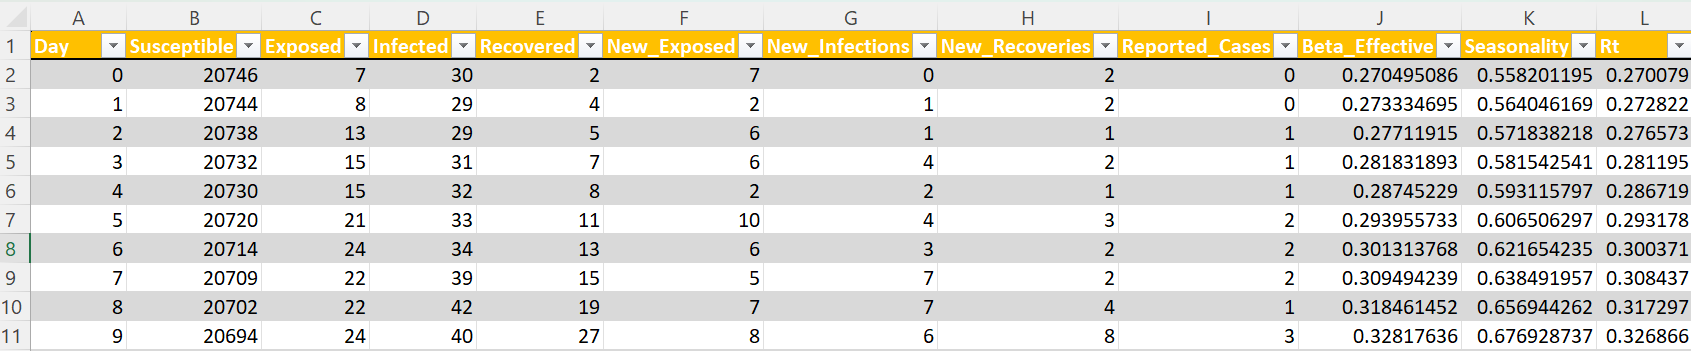
\includegraphics[width=0.8\linewidth]{Screenshot 2025-07-24 061221.png} 
    \caption{Dataset Snapshot from a random batch}
    \label{fig:my_figure}
\end{figure}
\begin{figure}[H] 
    \centering
    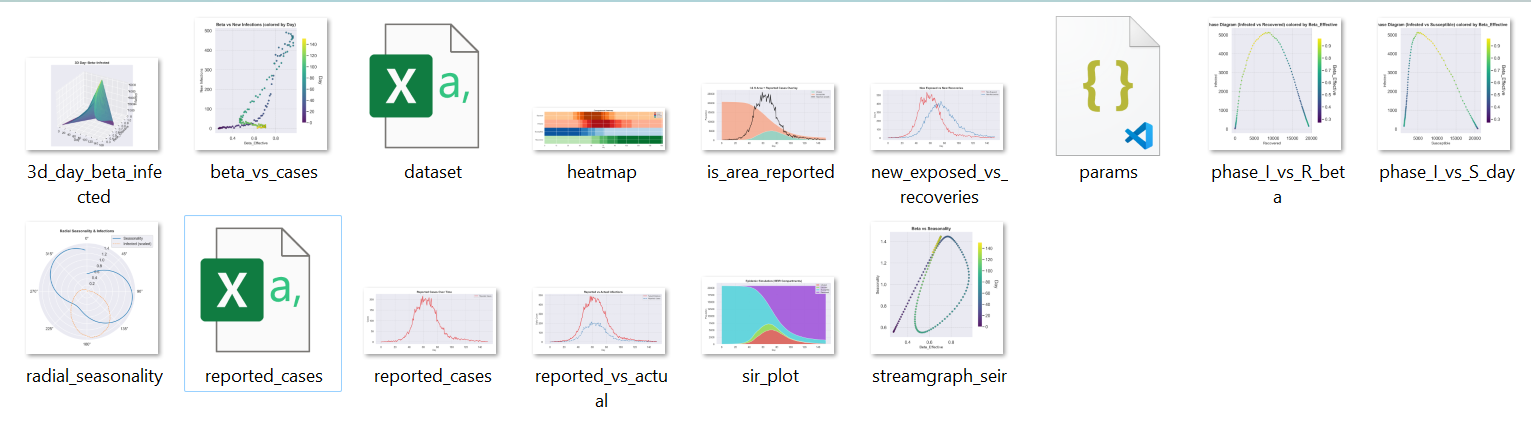
\includegraphics[width=0.8\linewidth]{Screenshot 2025-07-24 061312.png} 
    \caption{Directory snapshot of save CSVs, JSON and PNGs}
    \label{fig:my_figure}
\end{figure}
\textbf{Reproducibility and Logging}: reproduceibility is done by random seeds, this allows any experiment to be fully replicated or benchmarked until the user hasn't deleted the params.json file.
\section{Visual Plots and Demonstration}
Visual Plots are an integral part of BIGBOY1.2, it presents epidemic simulation data into interpretable and high dimensional plots. These visual plots could be used as analytical tools that could validate moedl outputs and also reveal deeper insights like epidemic progression, interventions and control
\subsection{Overview of the Plotting System}
Upon simulation, BIGBOY1.2 allows the users to generate a diverse set of set plots by passing --plots all or --plots sir. It has a modular plotting engine that allows both minimal and advanced visualization and the output is aved as high resolution PNG files. All of the plots are further save in timestamped directories with accompanying metadata, ensuring reporducibility.
\subsection{SEIR Compartment Plot}
A stacked area plot showing the progression of Susceptible (S), Exposed (S), Infected (I) adn Recovered (R) populations over time, classical SEIR-style visualization is foundational for understanding the macro level behavior of the epidemic. Th purpose of SEIR-stacked chart is revealing key phases such as exponential growth, peak infections and herd immnunity thresholds. 
\begin{figure}[H]
    \begin{minipage}{0.49\linewidth}
        \flushleft
        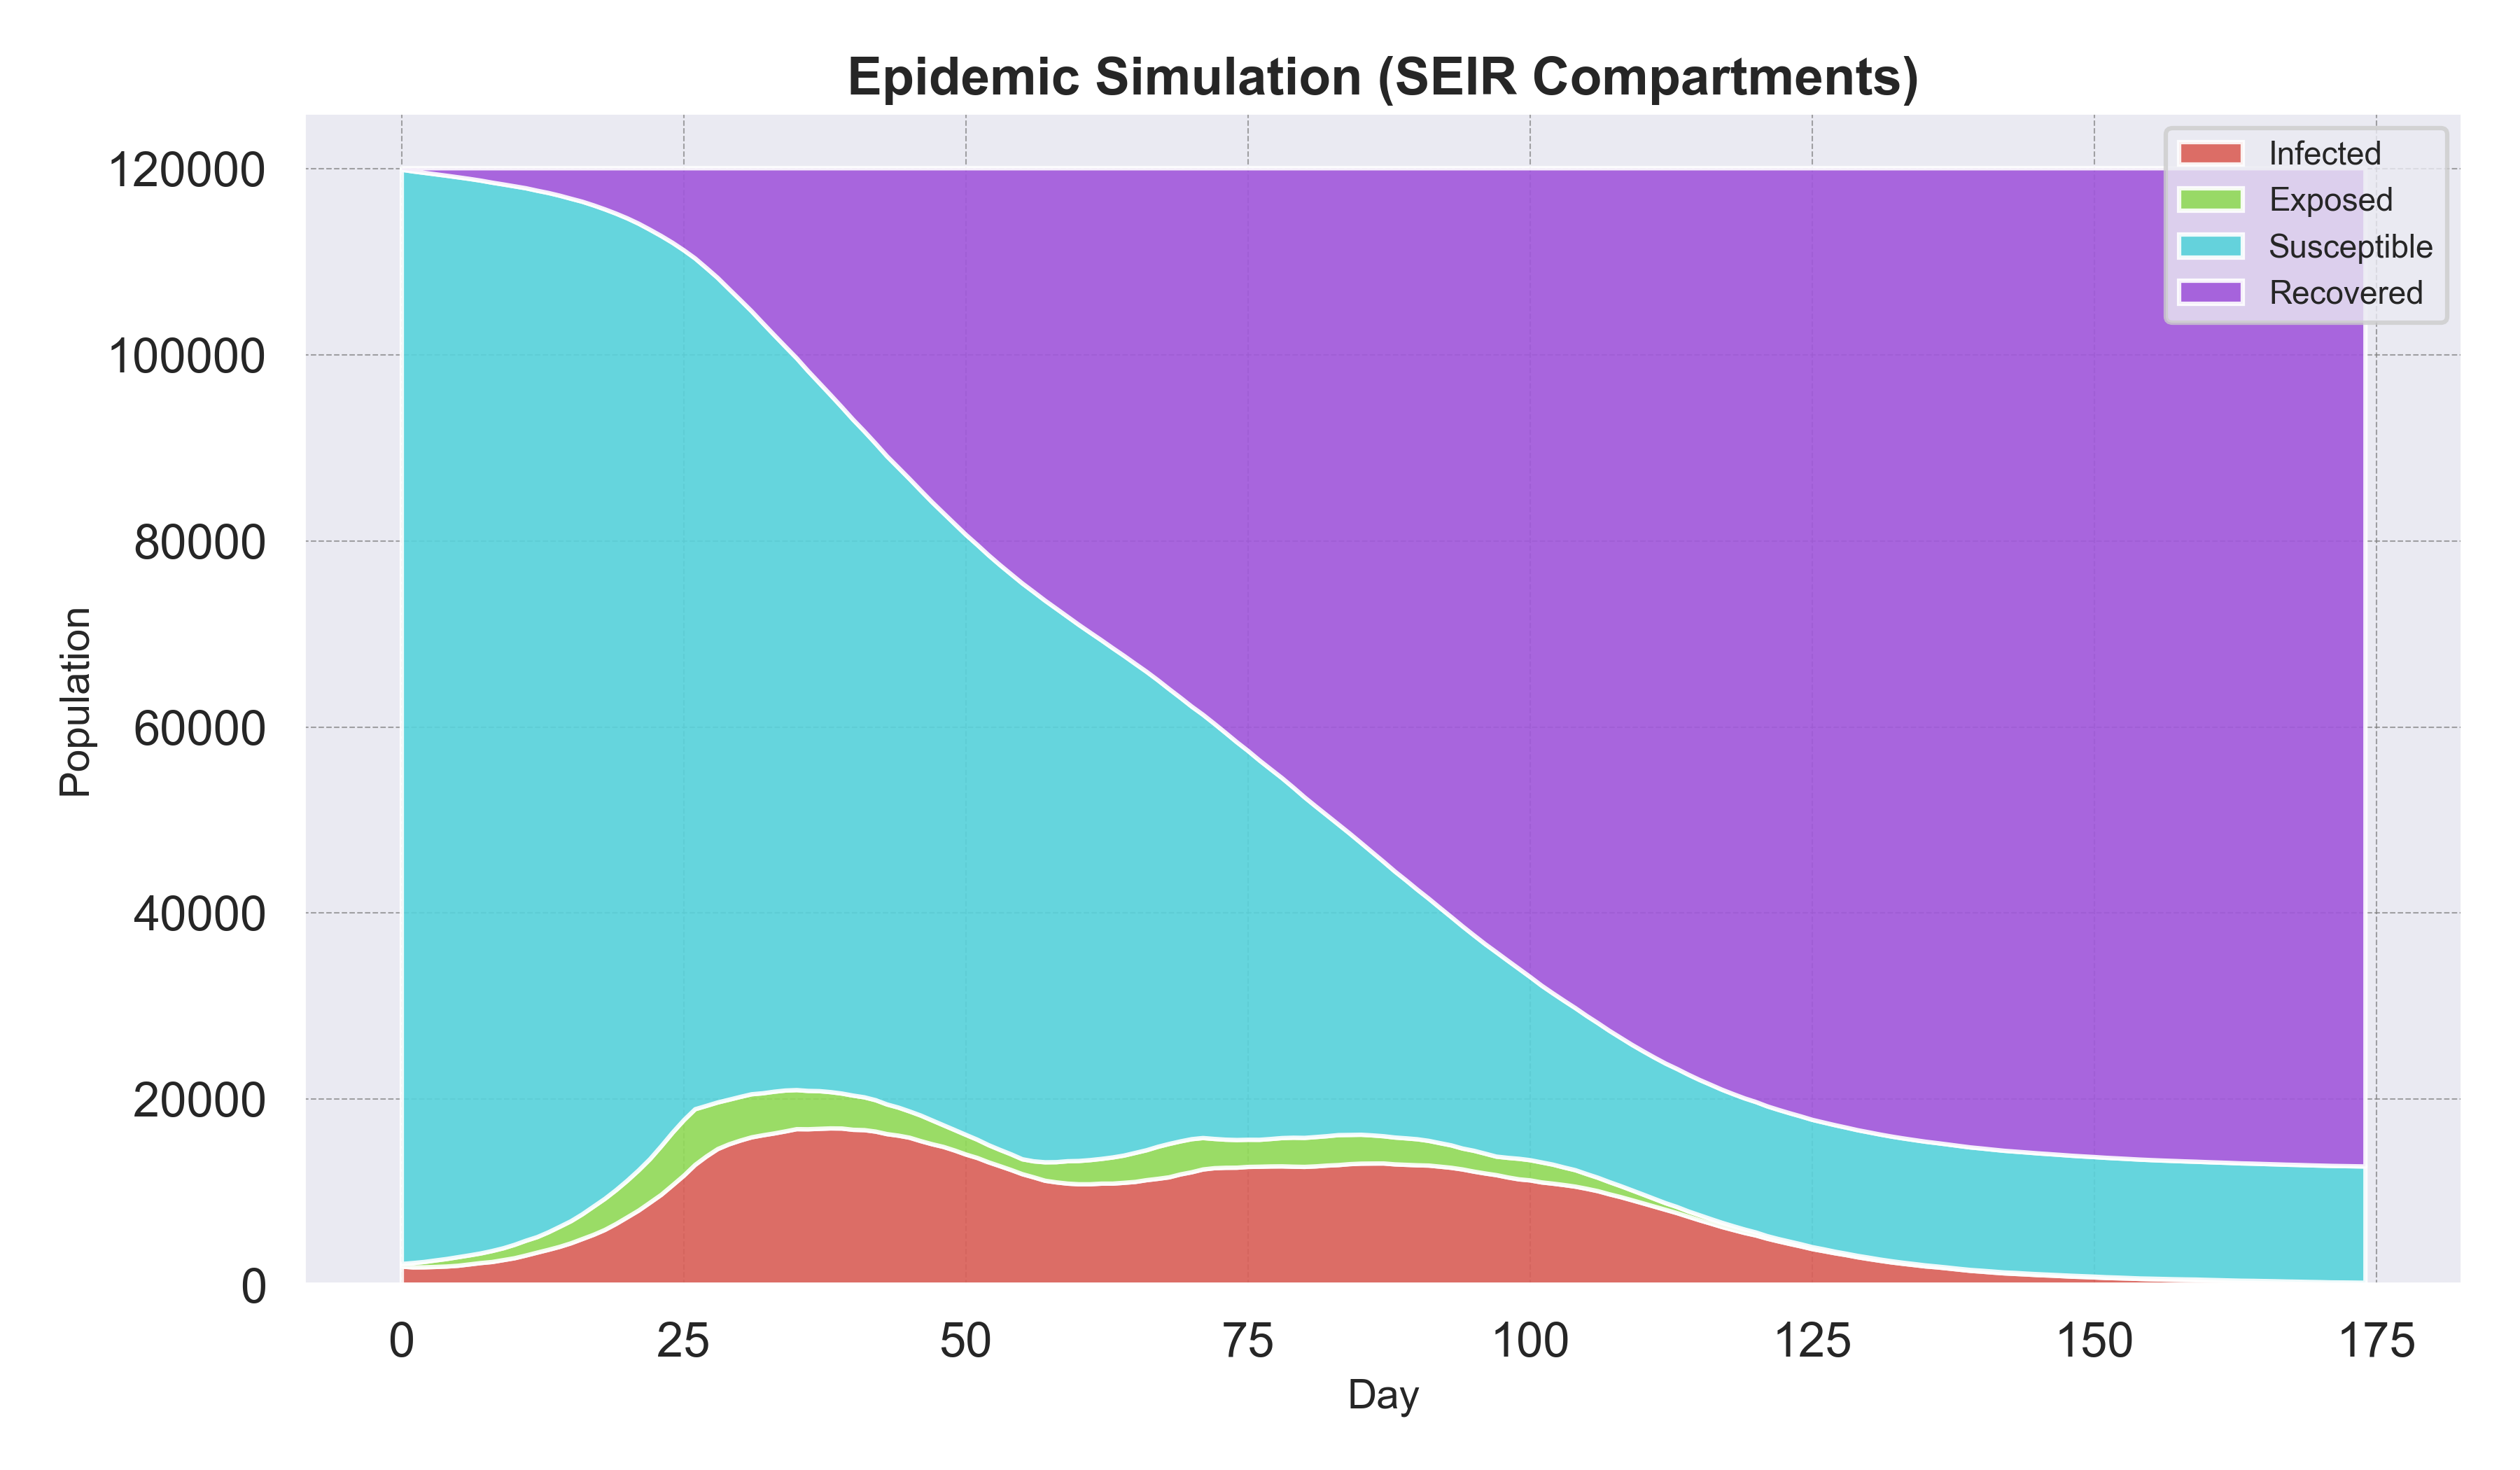
\includegraphics[width=\linewidth]{plotttt.png}
    \end{minipage}
    \hfill
    \begin{minipage}{0.49\linewidth}
        \flushright
        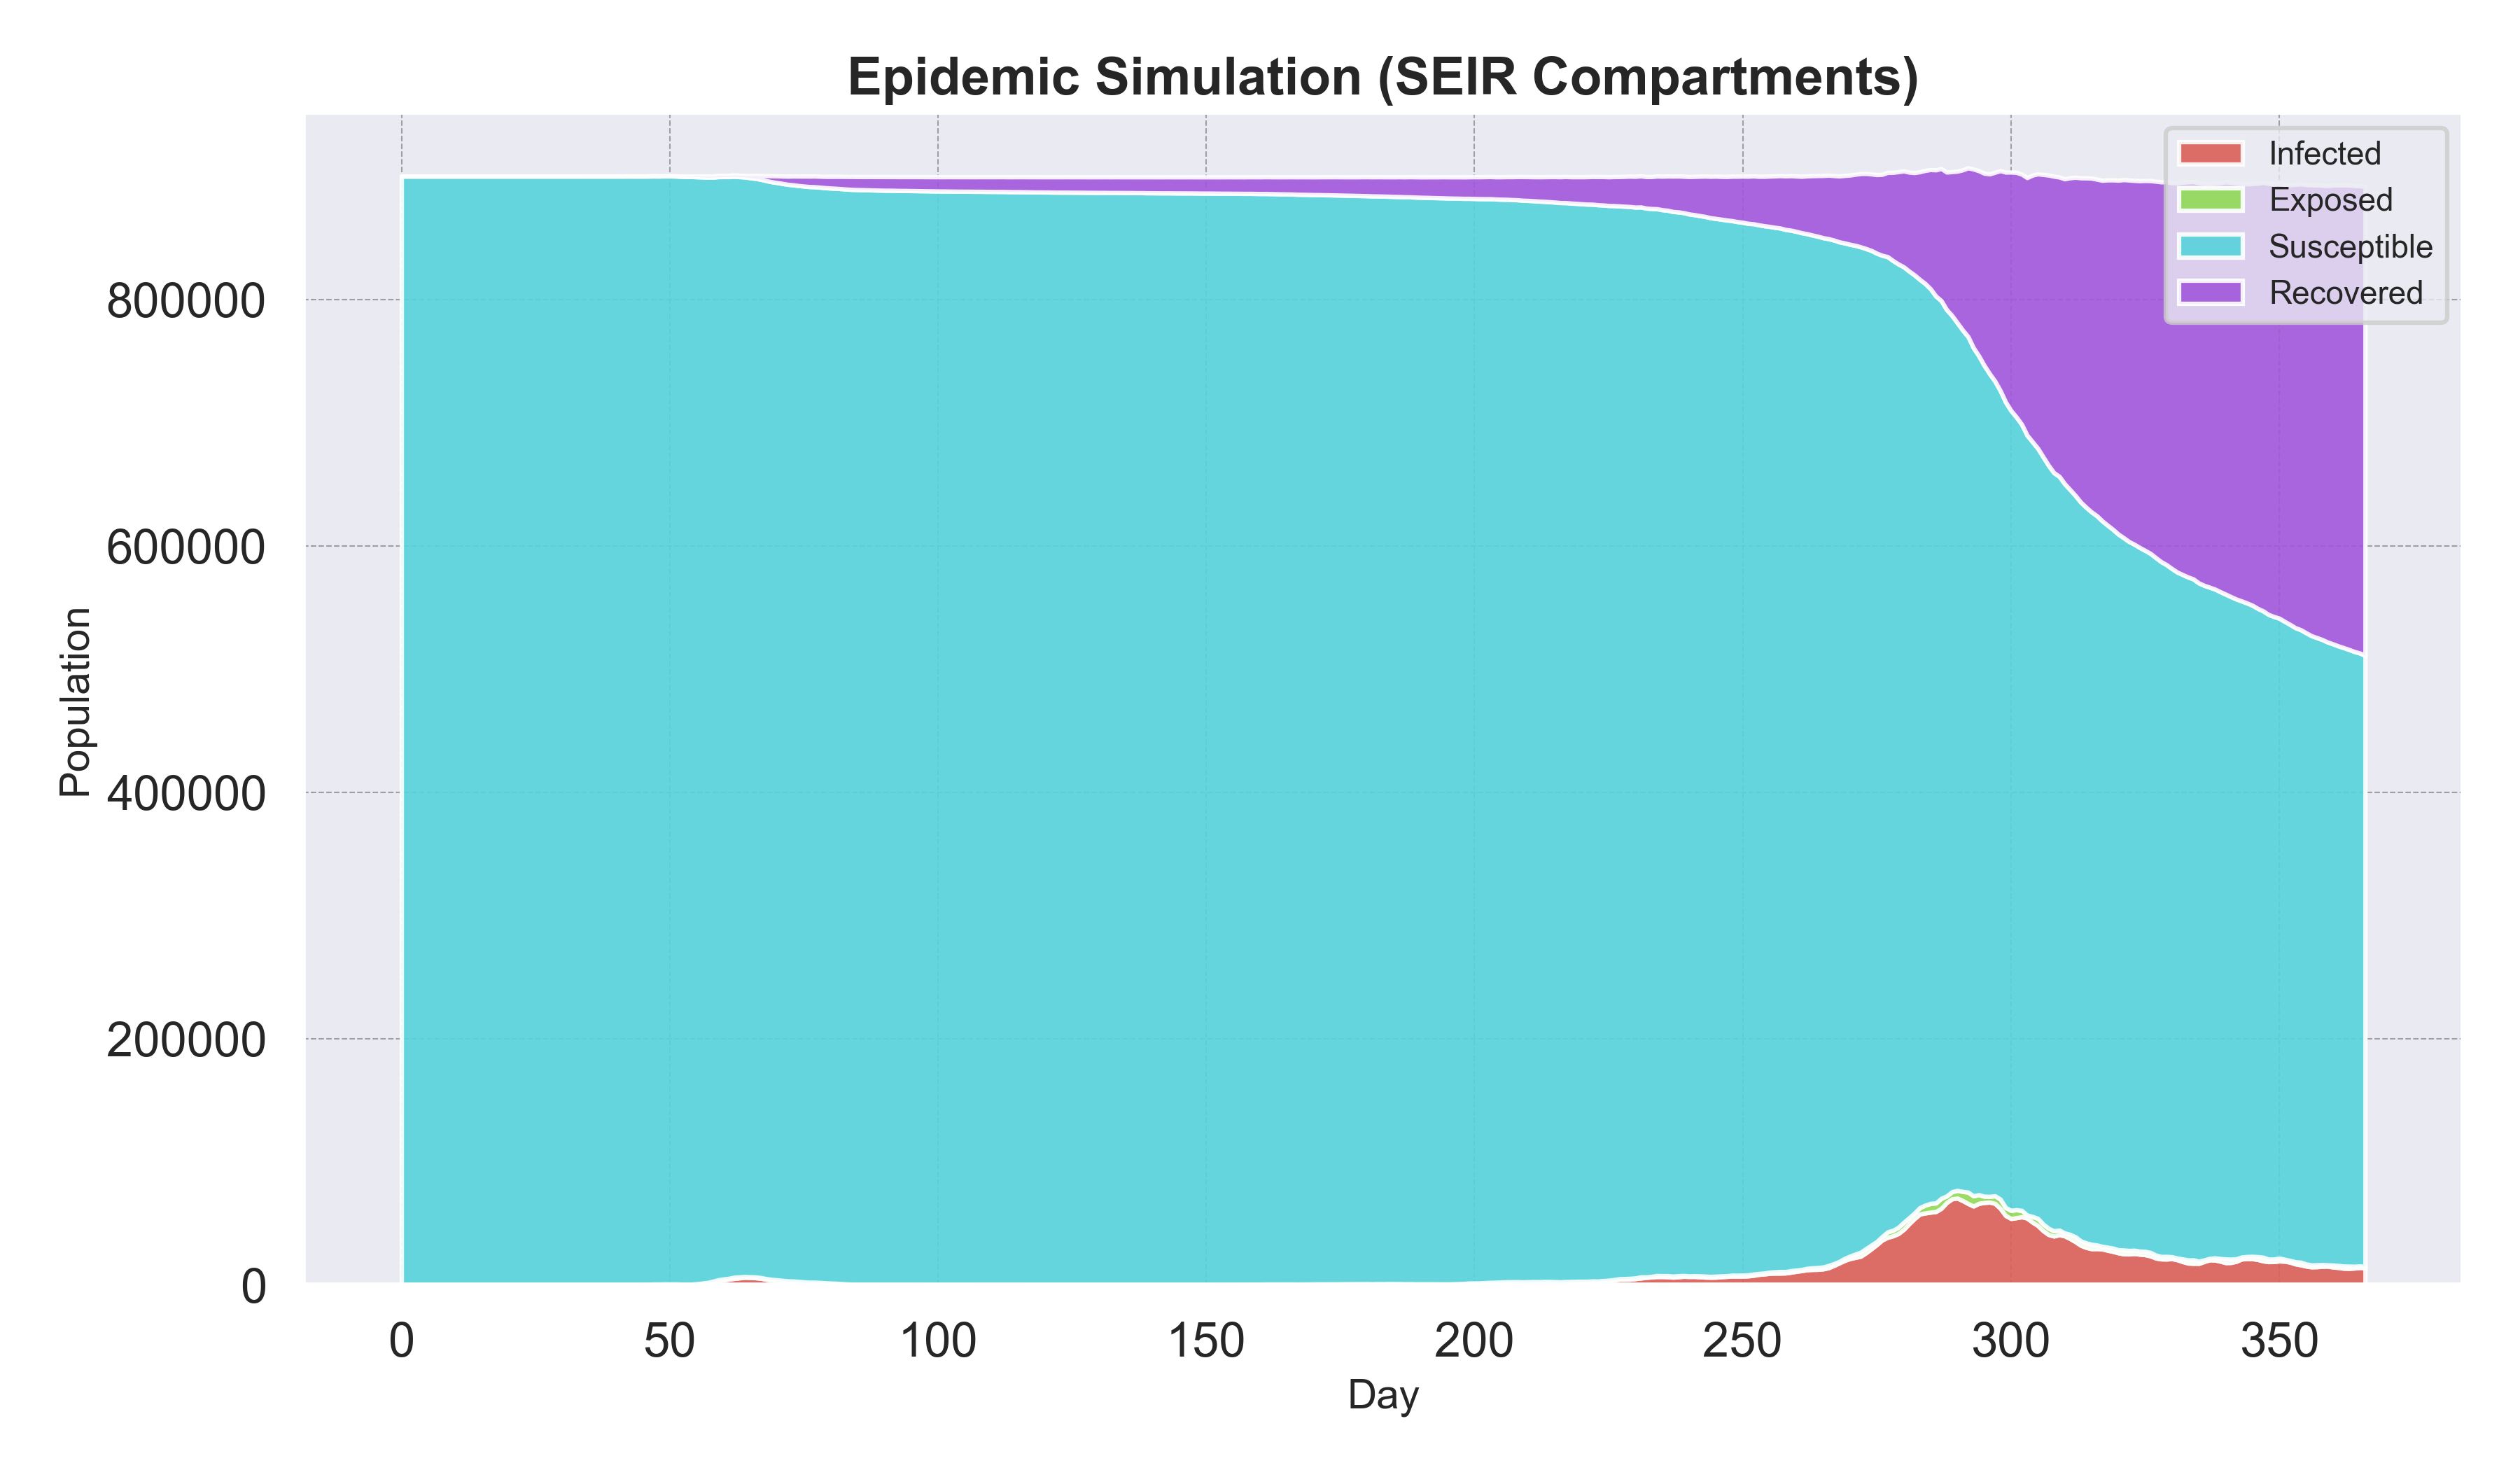
\includegraphics[width=\linewidth]{sir_plot.png}
    \end{minipage}
    
    \caption{SEIR stacked plots from a random batch}
    \label{fig:seir-side-by-side}
\end{figure}


\subsection{Reported Cases Timeline}
It displays the reported cases across days, this contracts the real world observed data with latent epidemic dynamics. It simulated the public health reporting pattern .
\begin{figure}[H]
    \begin{minipage}{0.49\linewidth}
        \flushleft
        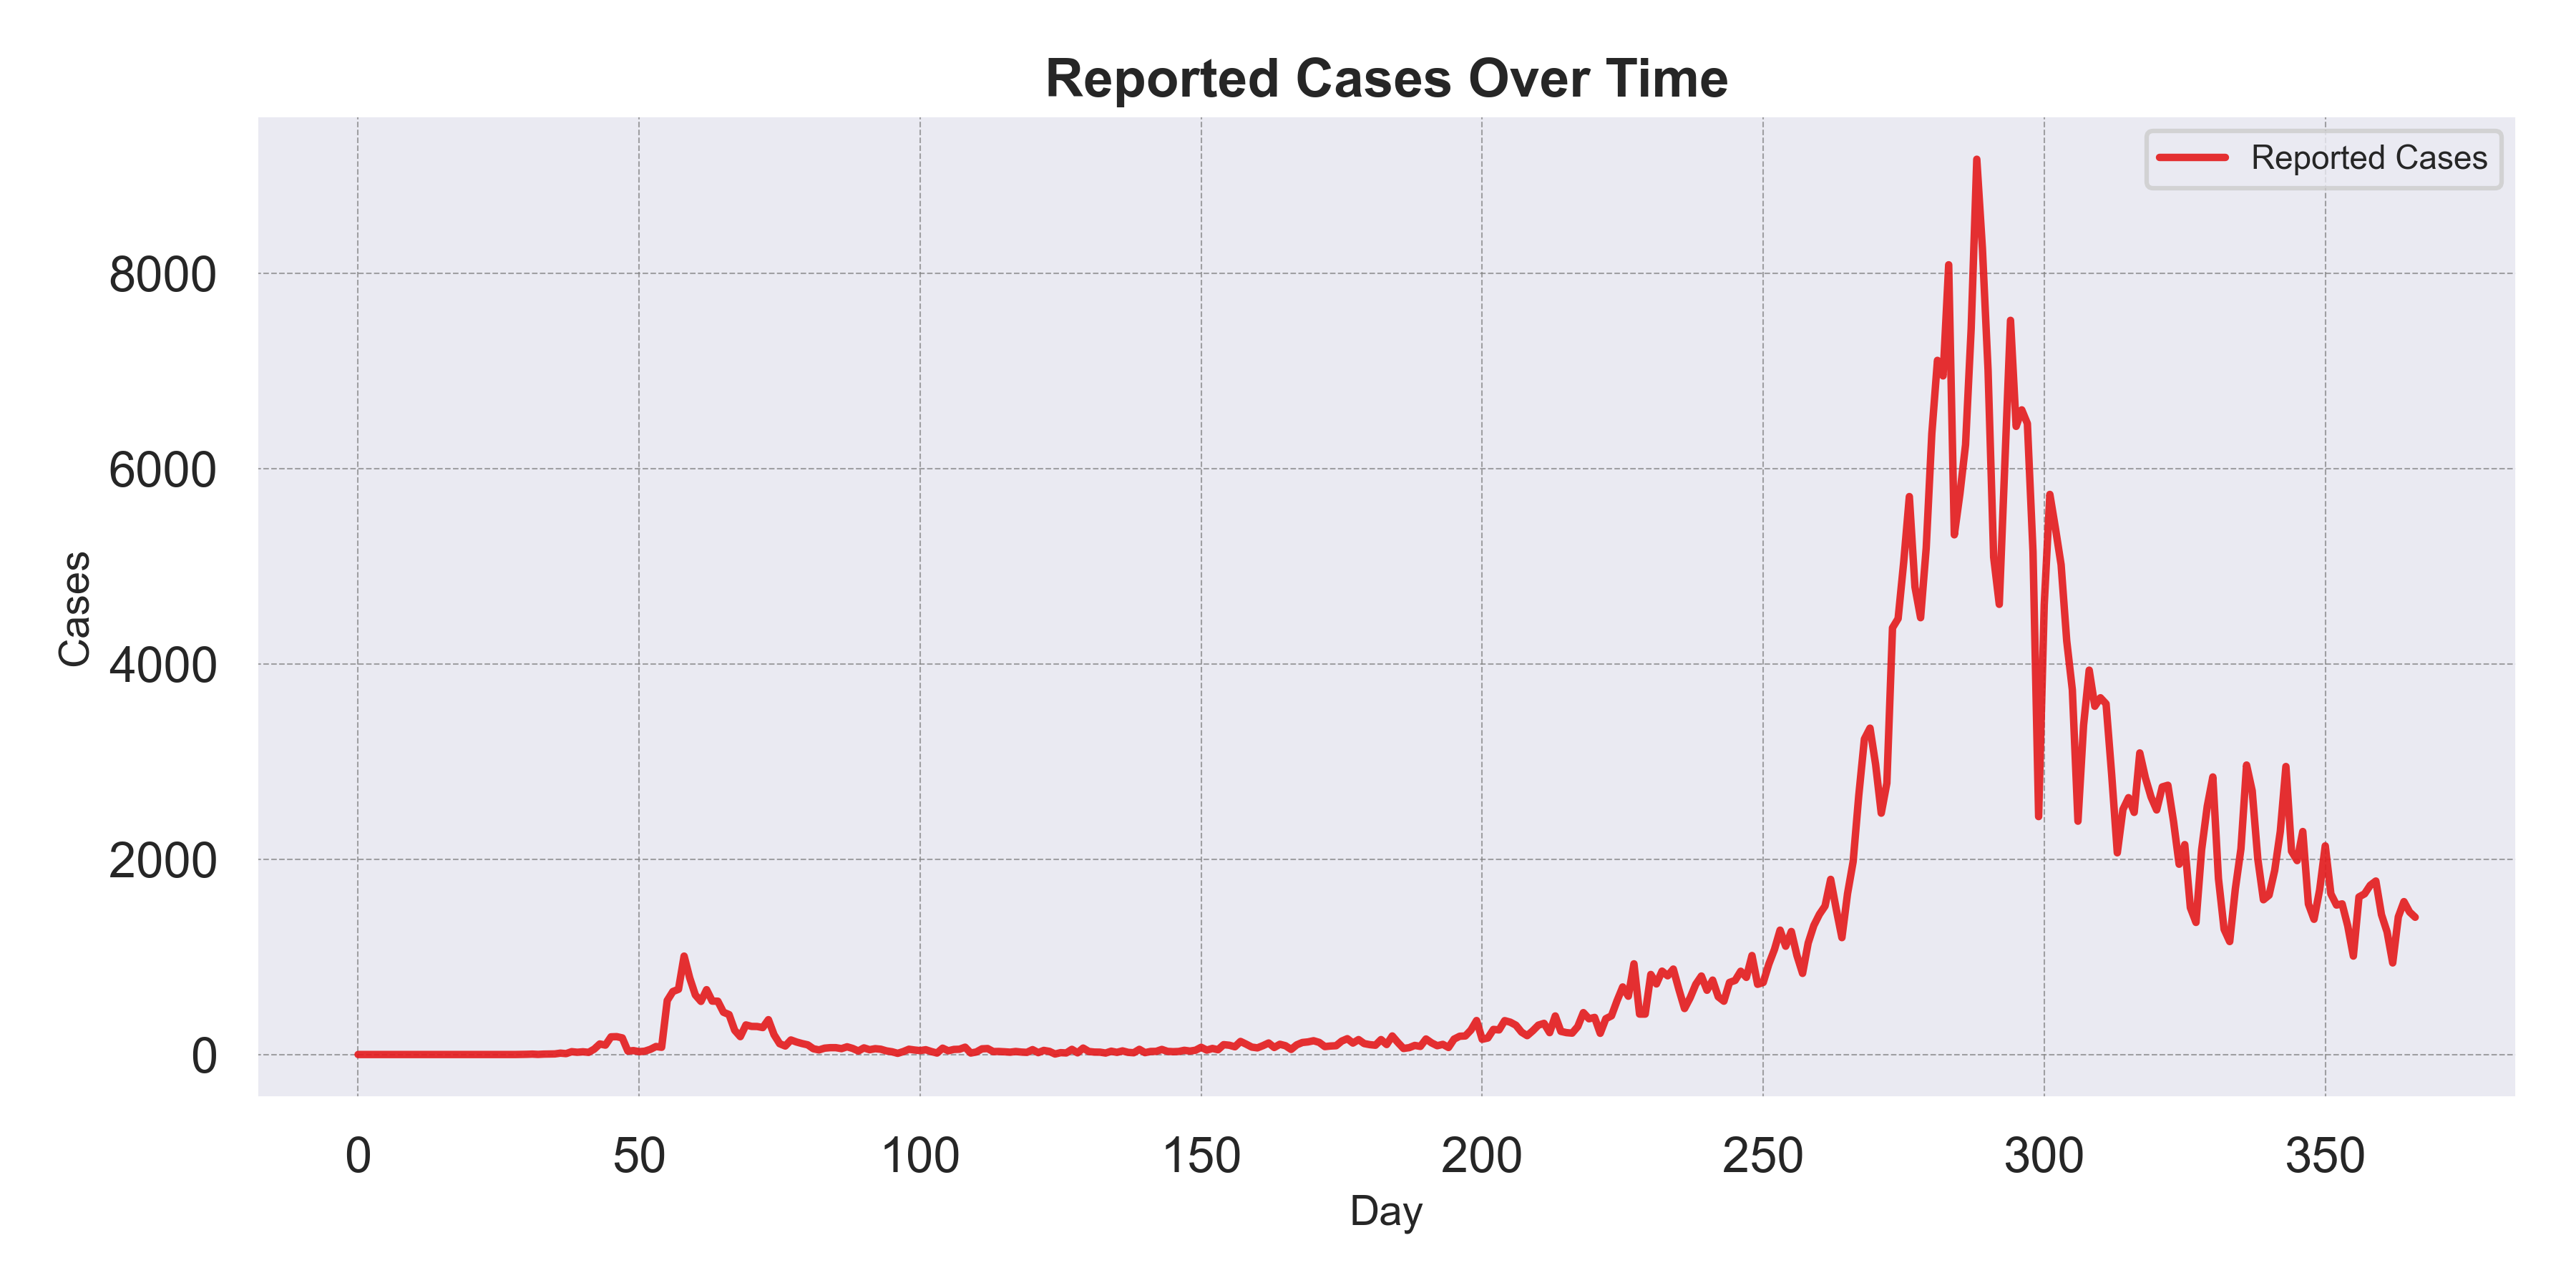
\includegraphics[width=\linewidth]{reported_cases.png}
    \end{minipage}
    \hfill
    \begin{minipage}{0.49\linewidth}
        \flushright
        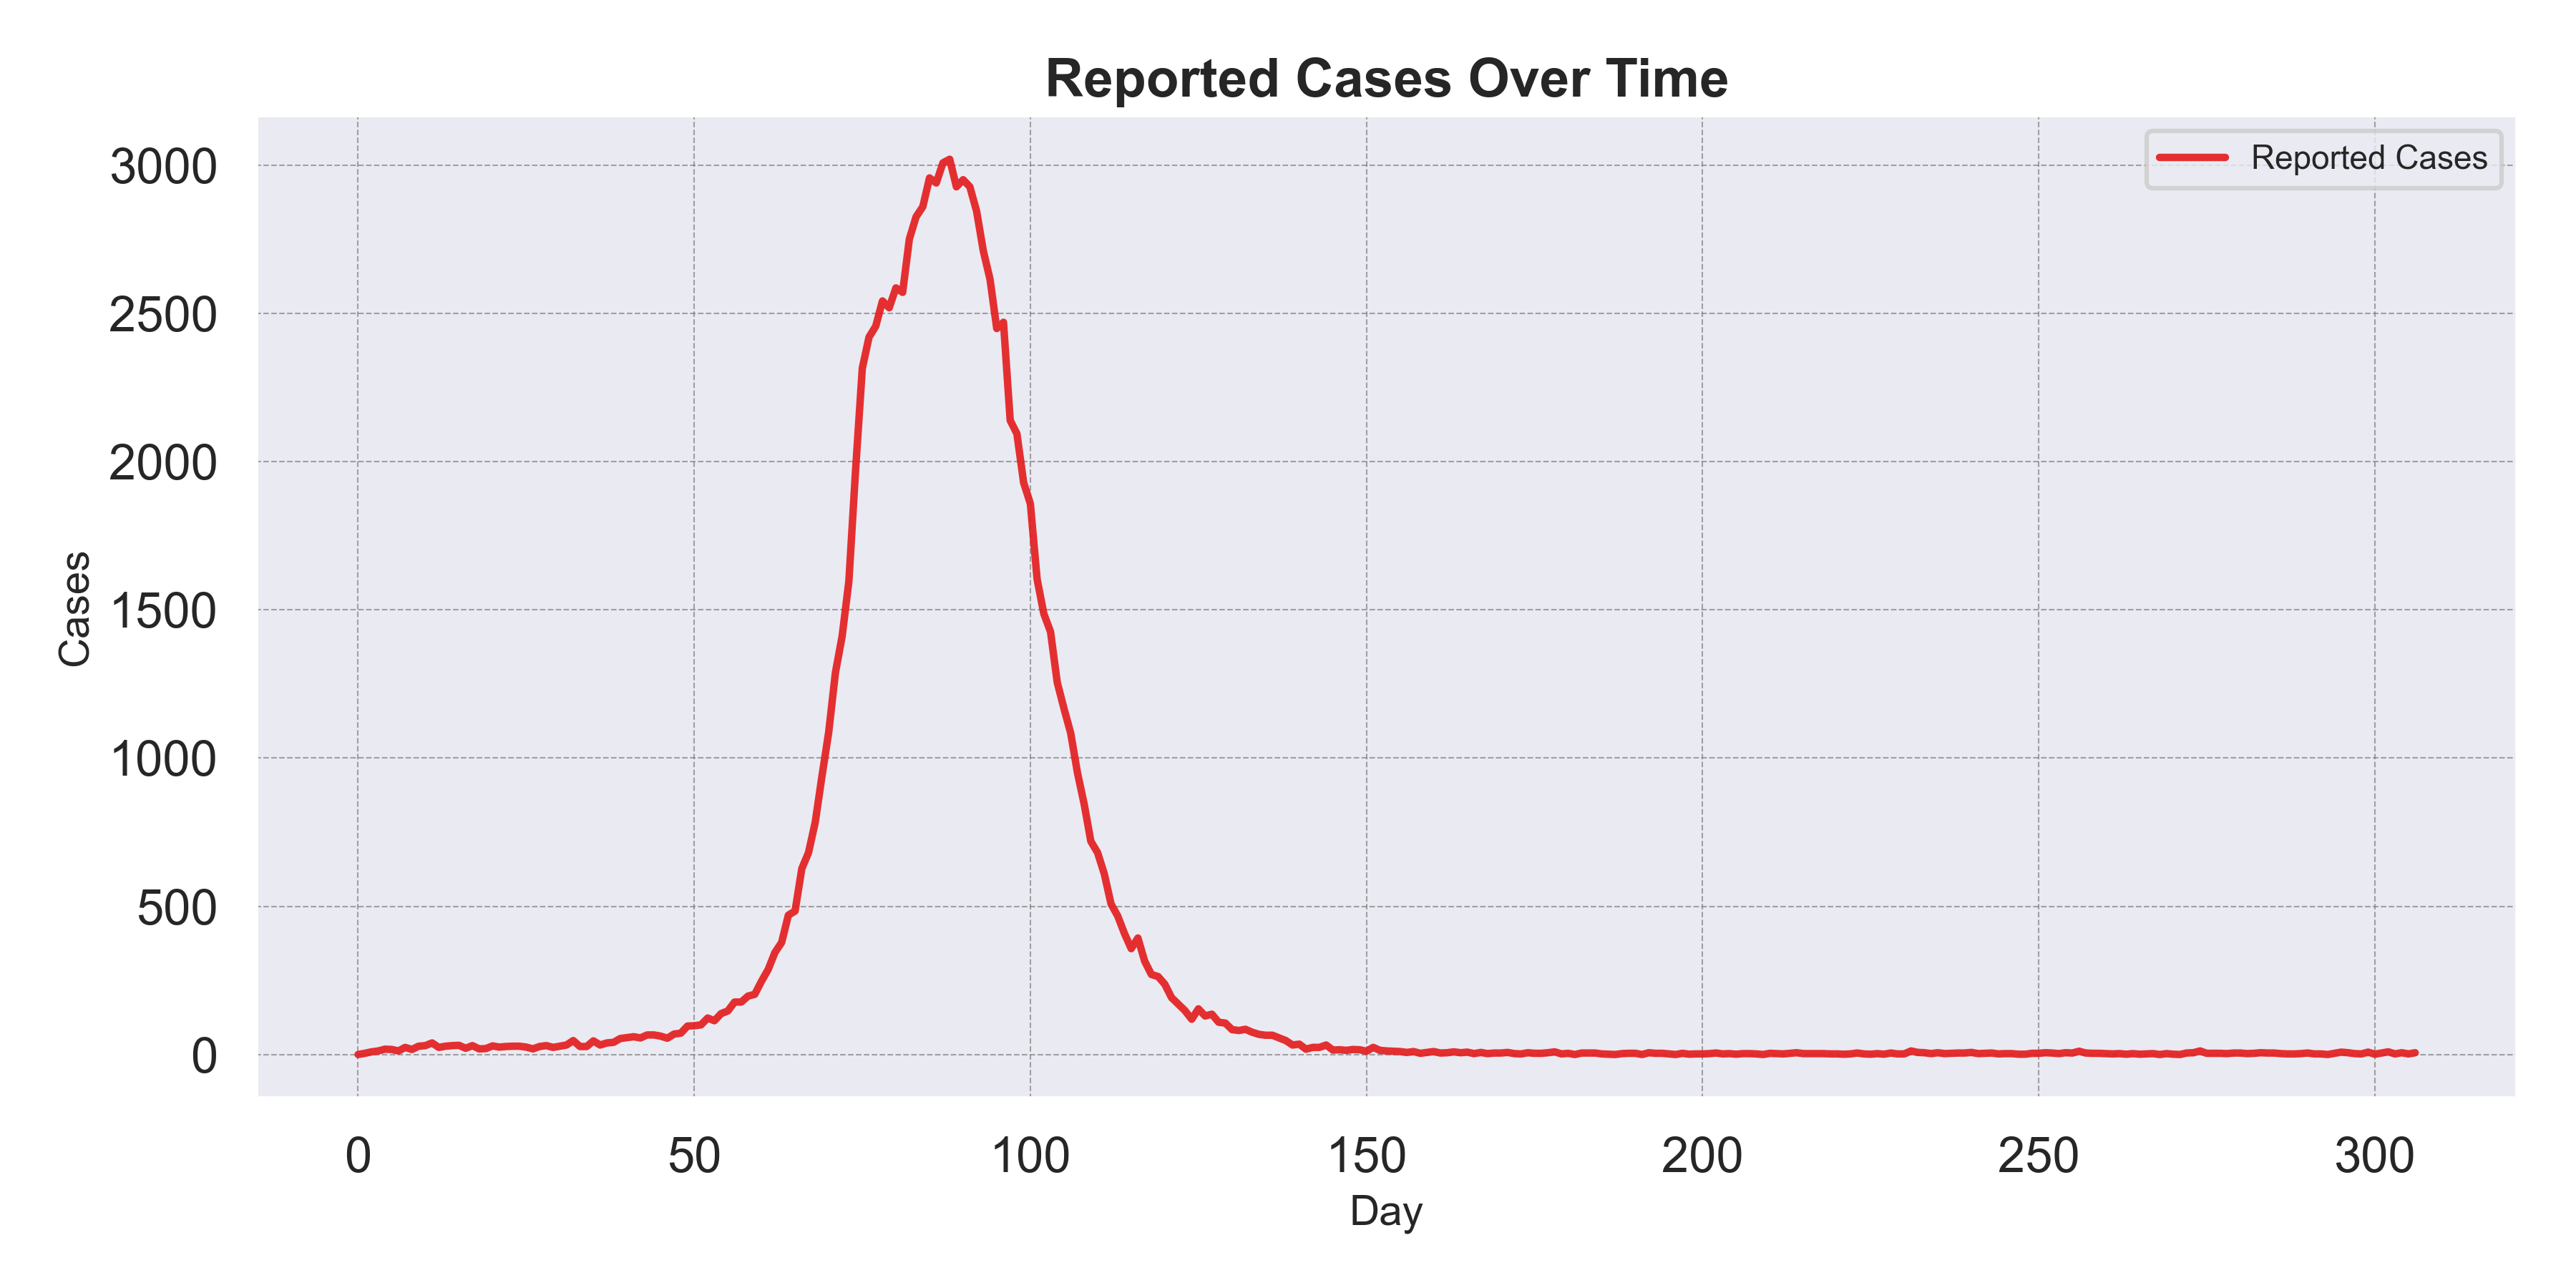
\includegraphics[width=\linewidth]{renama.png}
    \end{minipage}
    
    \caption{Reported cases from a random batch}
    \label{fig:seir-side-by-side}
\end{figure}

\subsection{3D plot of \text{day} \times $\beta$ \times \text{infection}}
This 3D plot displays how contagious a disease is, as contingency and number of infections are not linear, 3D visualization shows how small changes in $\beta$ can lead to explosive outbreaks under conditions. Lag effects can also be revealed visualizing this 3D plot, even if $\beta$ rises sharply, infections may spike few days later, this helps in understadning incubation periods. \\
If an intervention like mask adherence is applied (or lockdown) , it causes $\beta$ to drop and the flattening infection counts could be seen in the Z-axis. This shows casual evidence of policy effectiveness in time. In multiple wave simulations, the 3D plot clearly shows how subsequent waves differ in timing, strength and transmissibility. These could be compared early vs later variants of the disease visually. 
\begin{figure}[H]
    \begin{minipage}{0.49\linewidth}
        \flushleft
        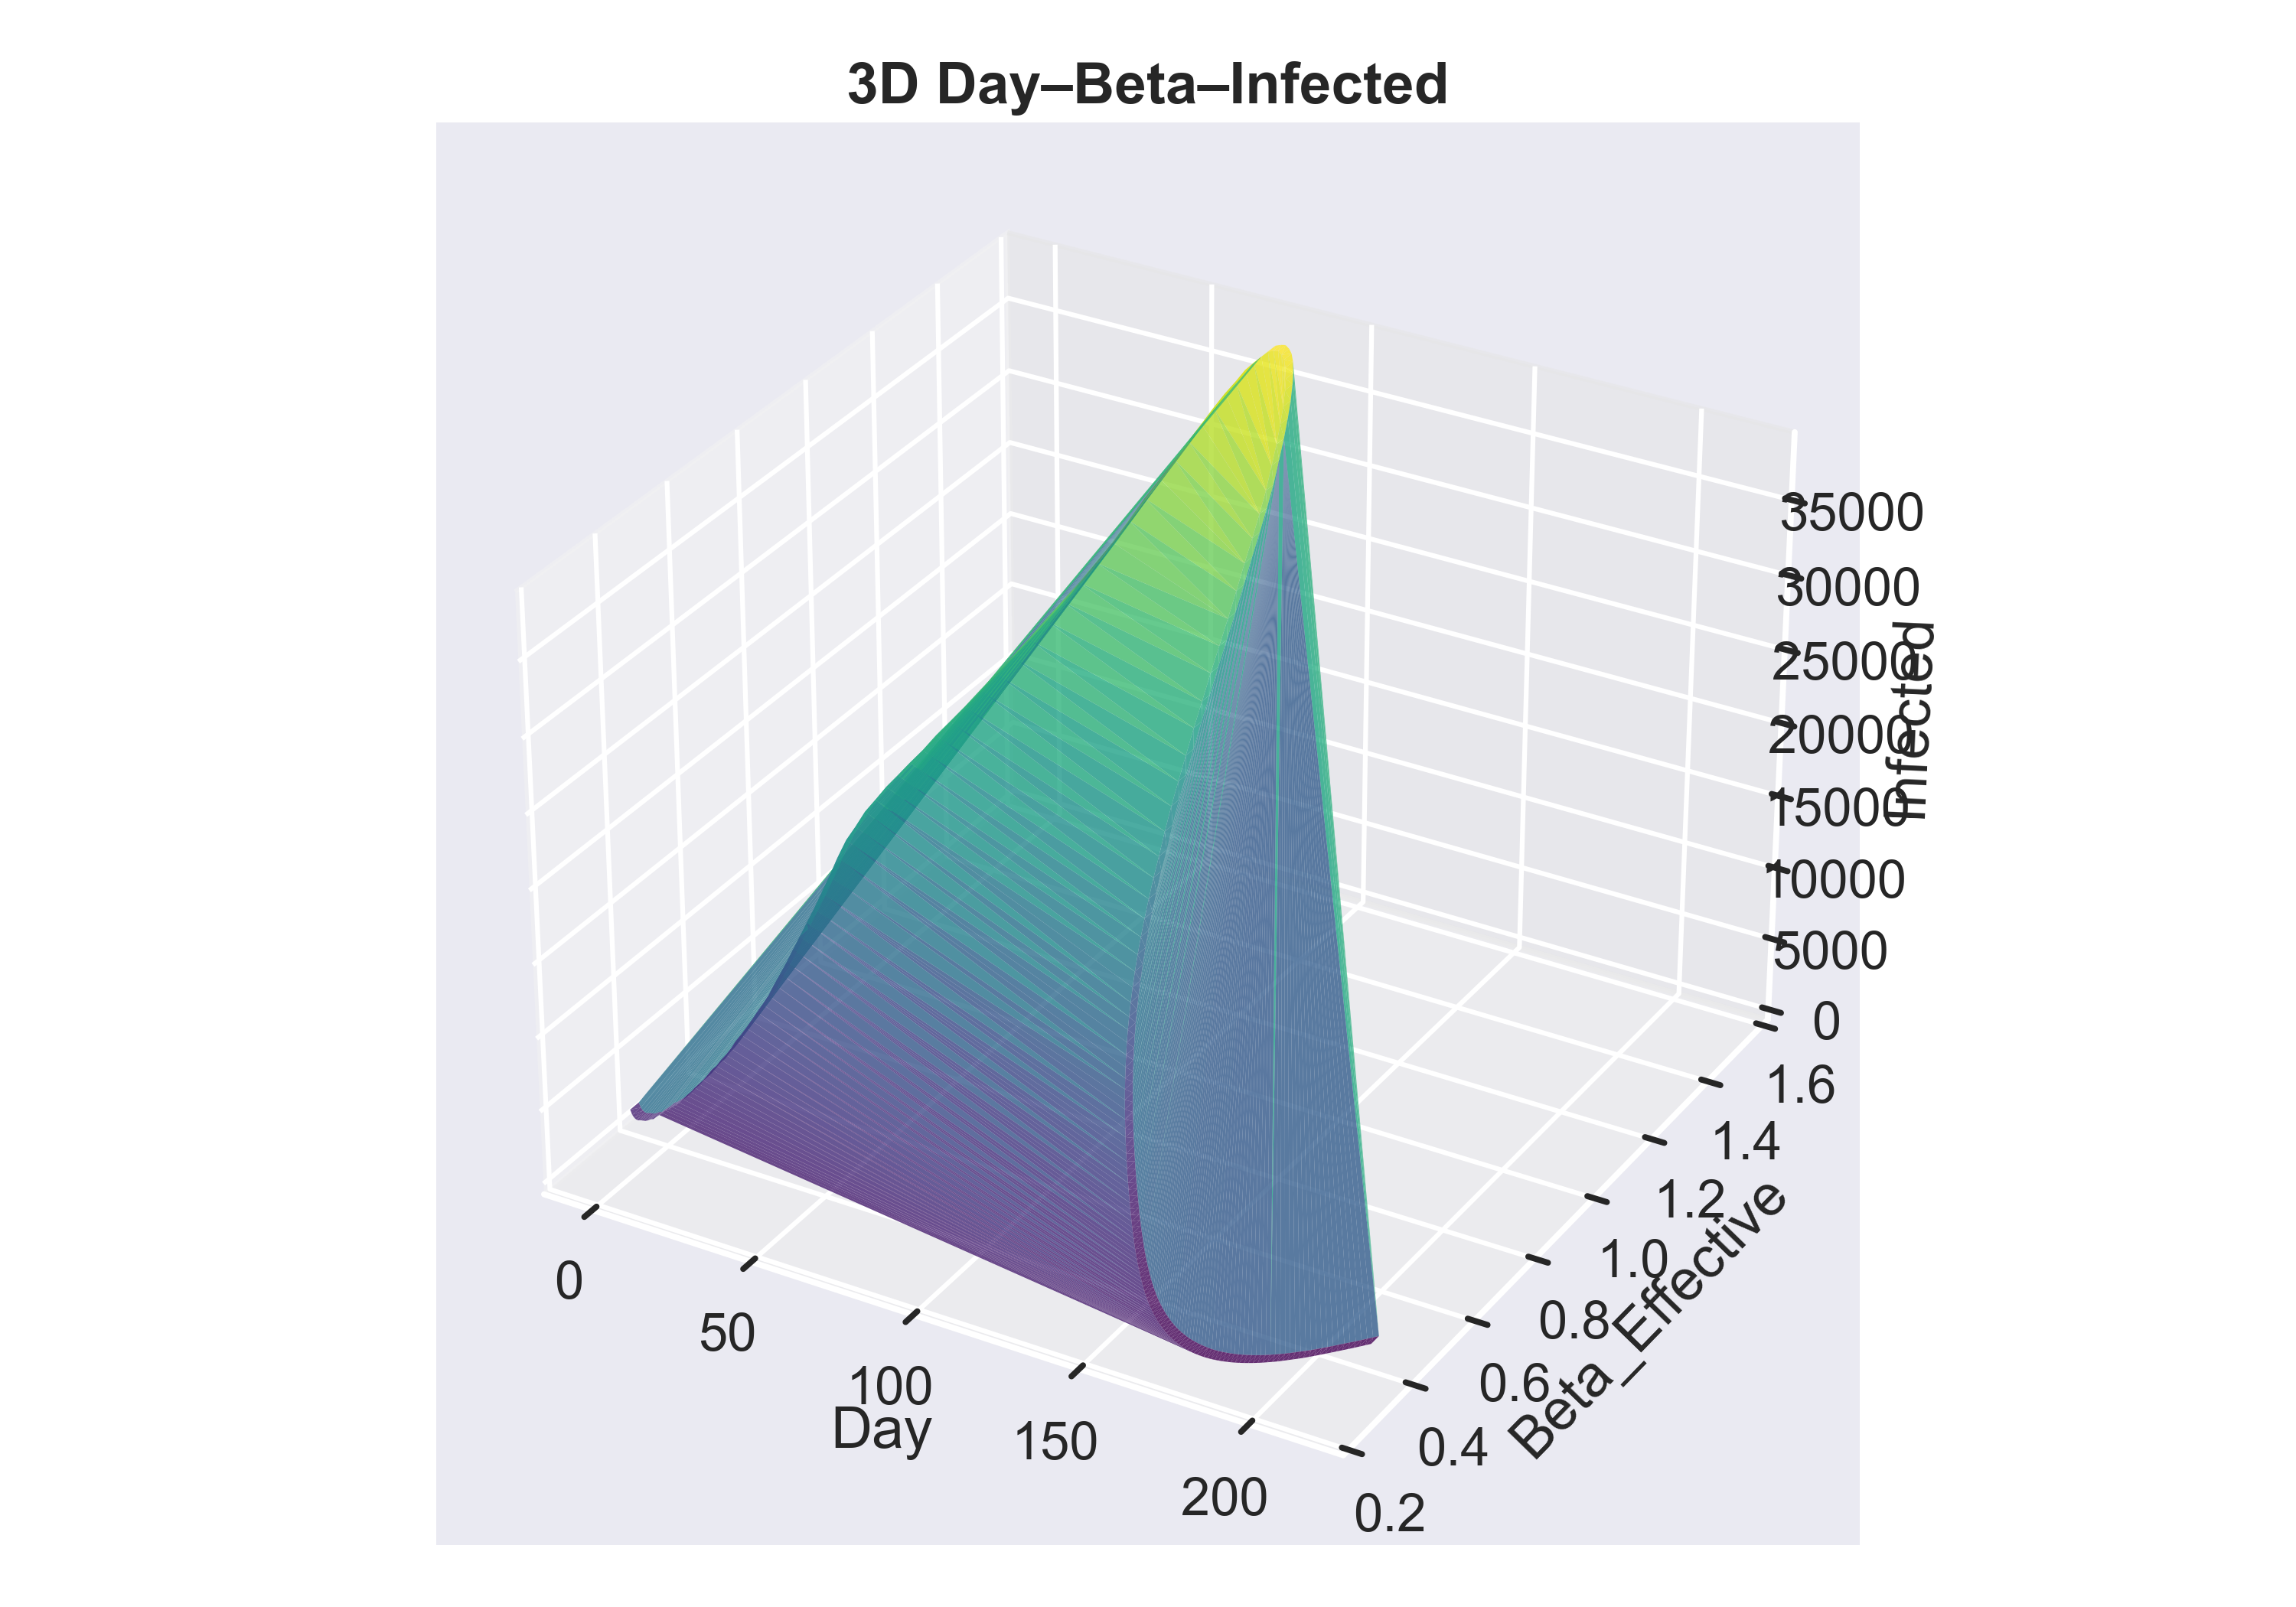
\includegraphics[width=\linewidth]{3d_day_beta_infected.png}
    \end{minipage}
    \hfill
    \begin{minipage}{0.49\linewidth}
        \flushright
        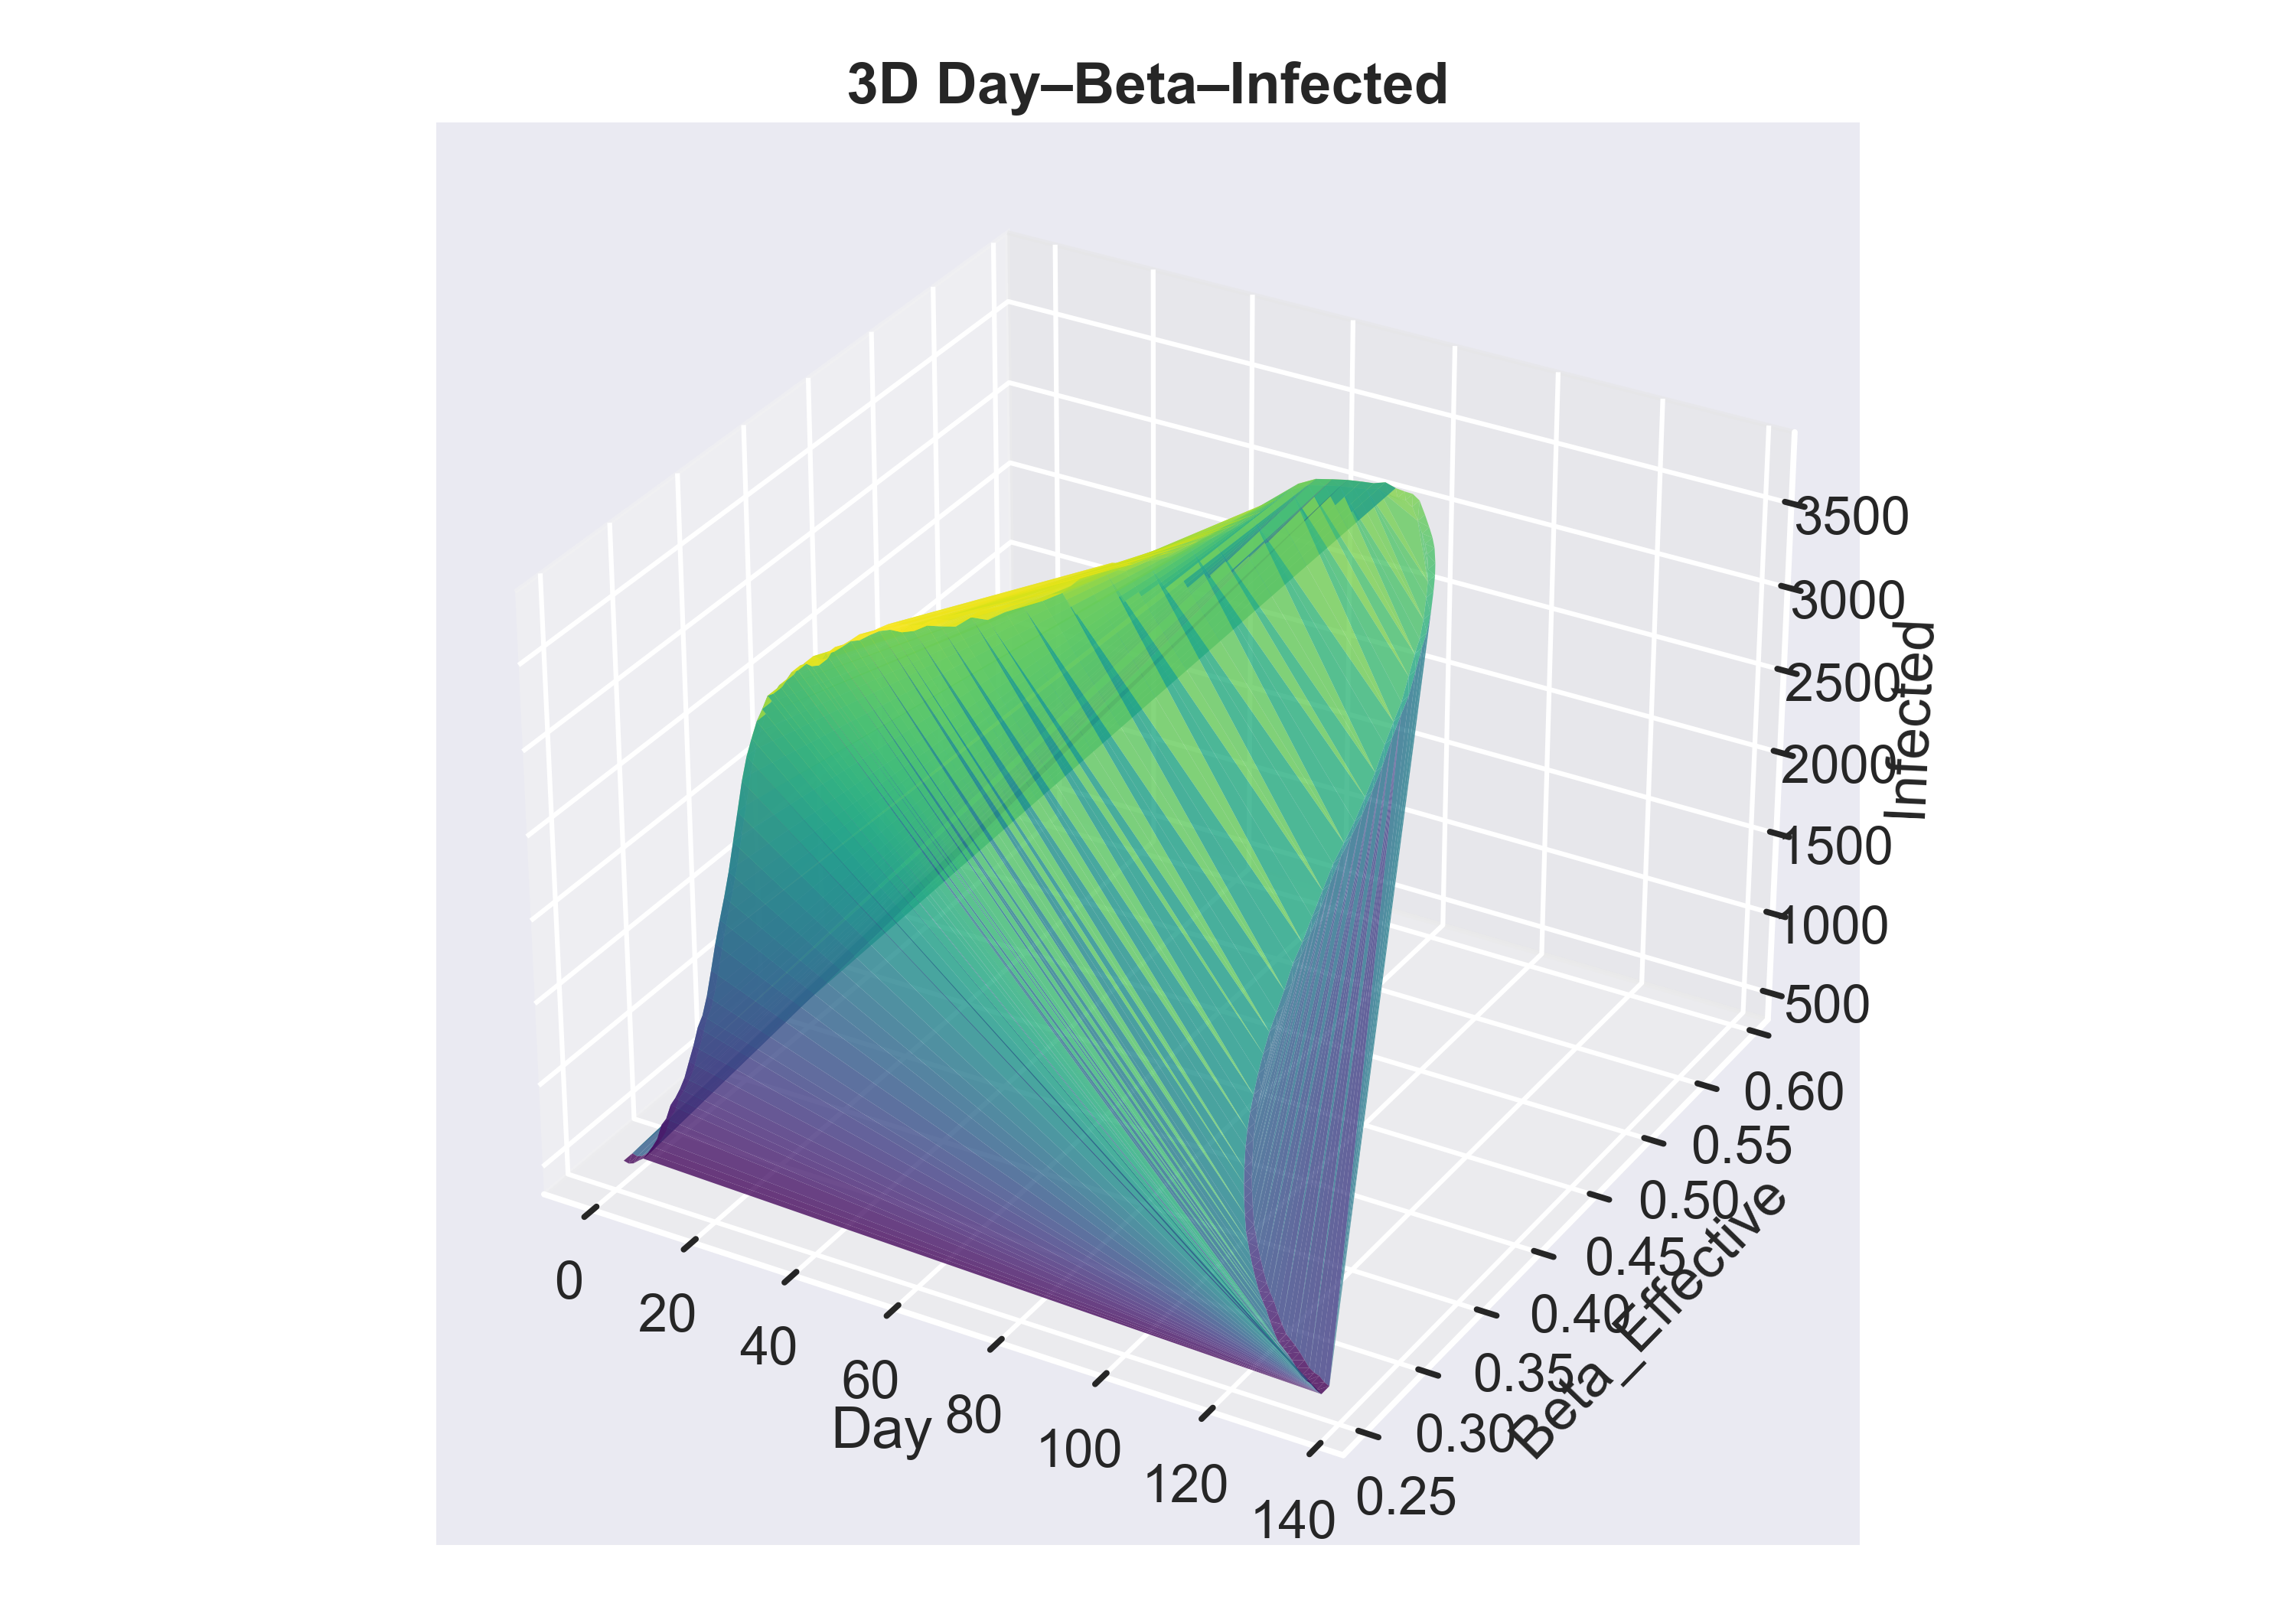
\includegraphics[width=\linewidth]{chnag.png}
    \end{minipage}
    
    \caption{3D plots from a random batch}
    \label{fig:seir-side-by-side}
\end{figure}
\subsection{$\beta$ vs. New Infections (Colored by Day)}
This scatterplot is crucial for understadning how chnages in $\beta$ correlate with spikes or drops in new infections. Higher $\beta$ generally increases the infections, but during later stanges, even higher $\beta$ may not cause spikes due to immunity build up. These effects are shown by Day, the scatter dots are colored by day.
\begin{figure}[H]
    \begin{minipage}{0.49\linewidth}
        \flushleft
        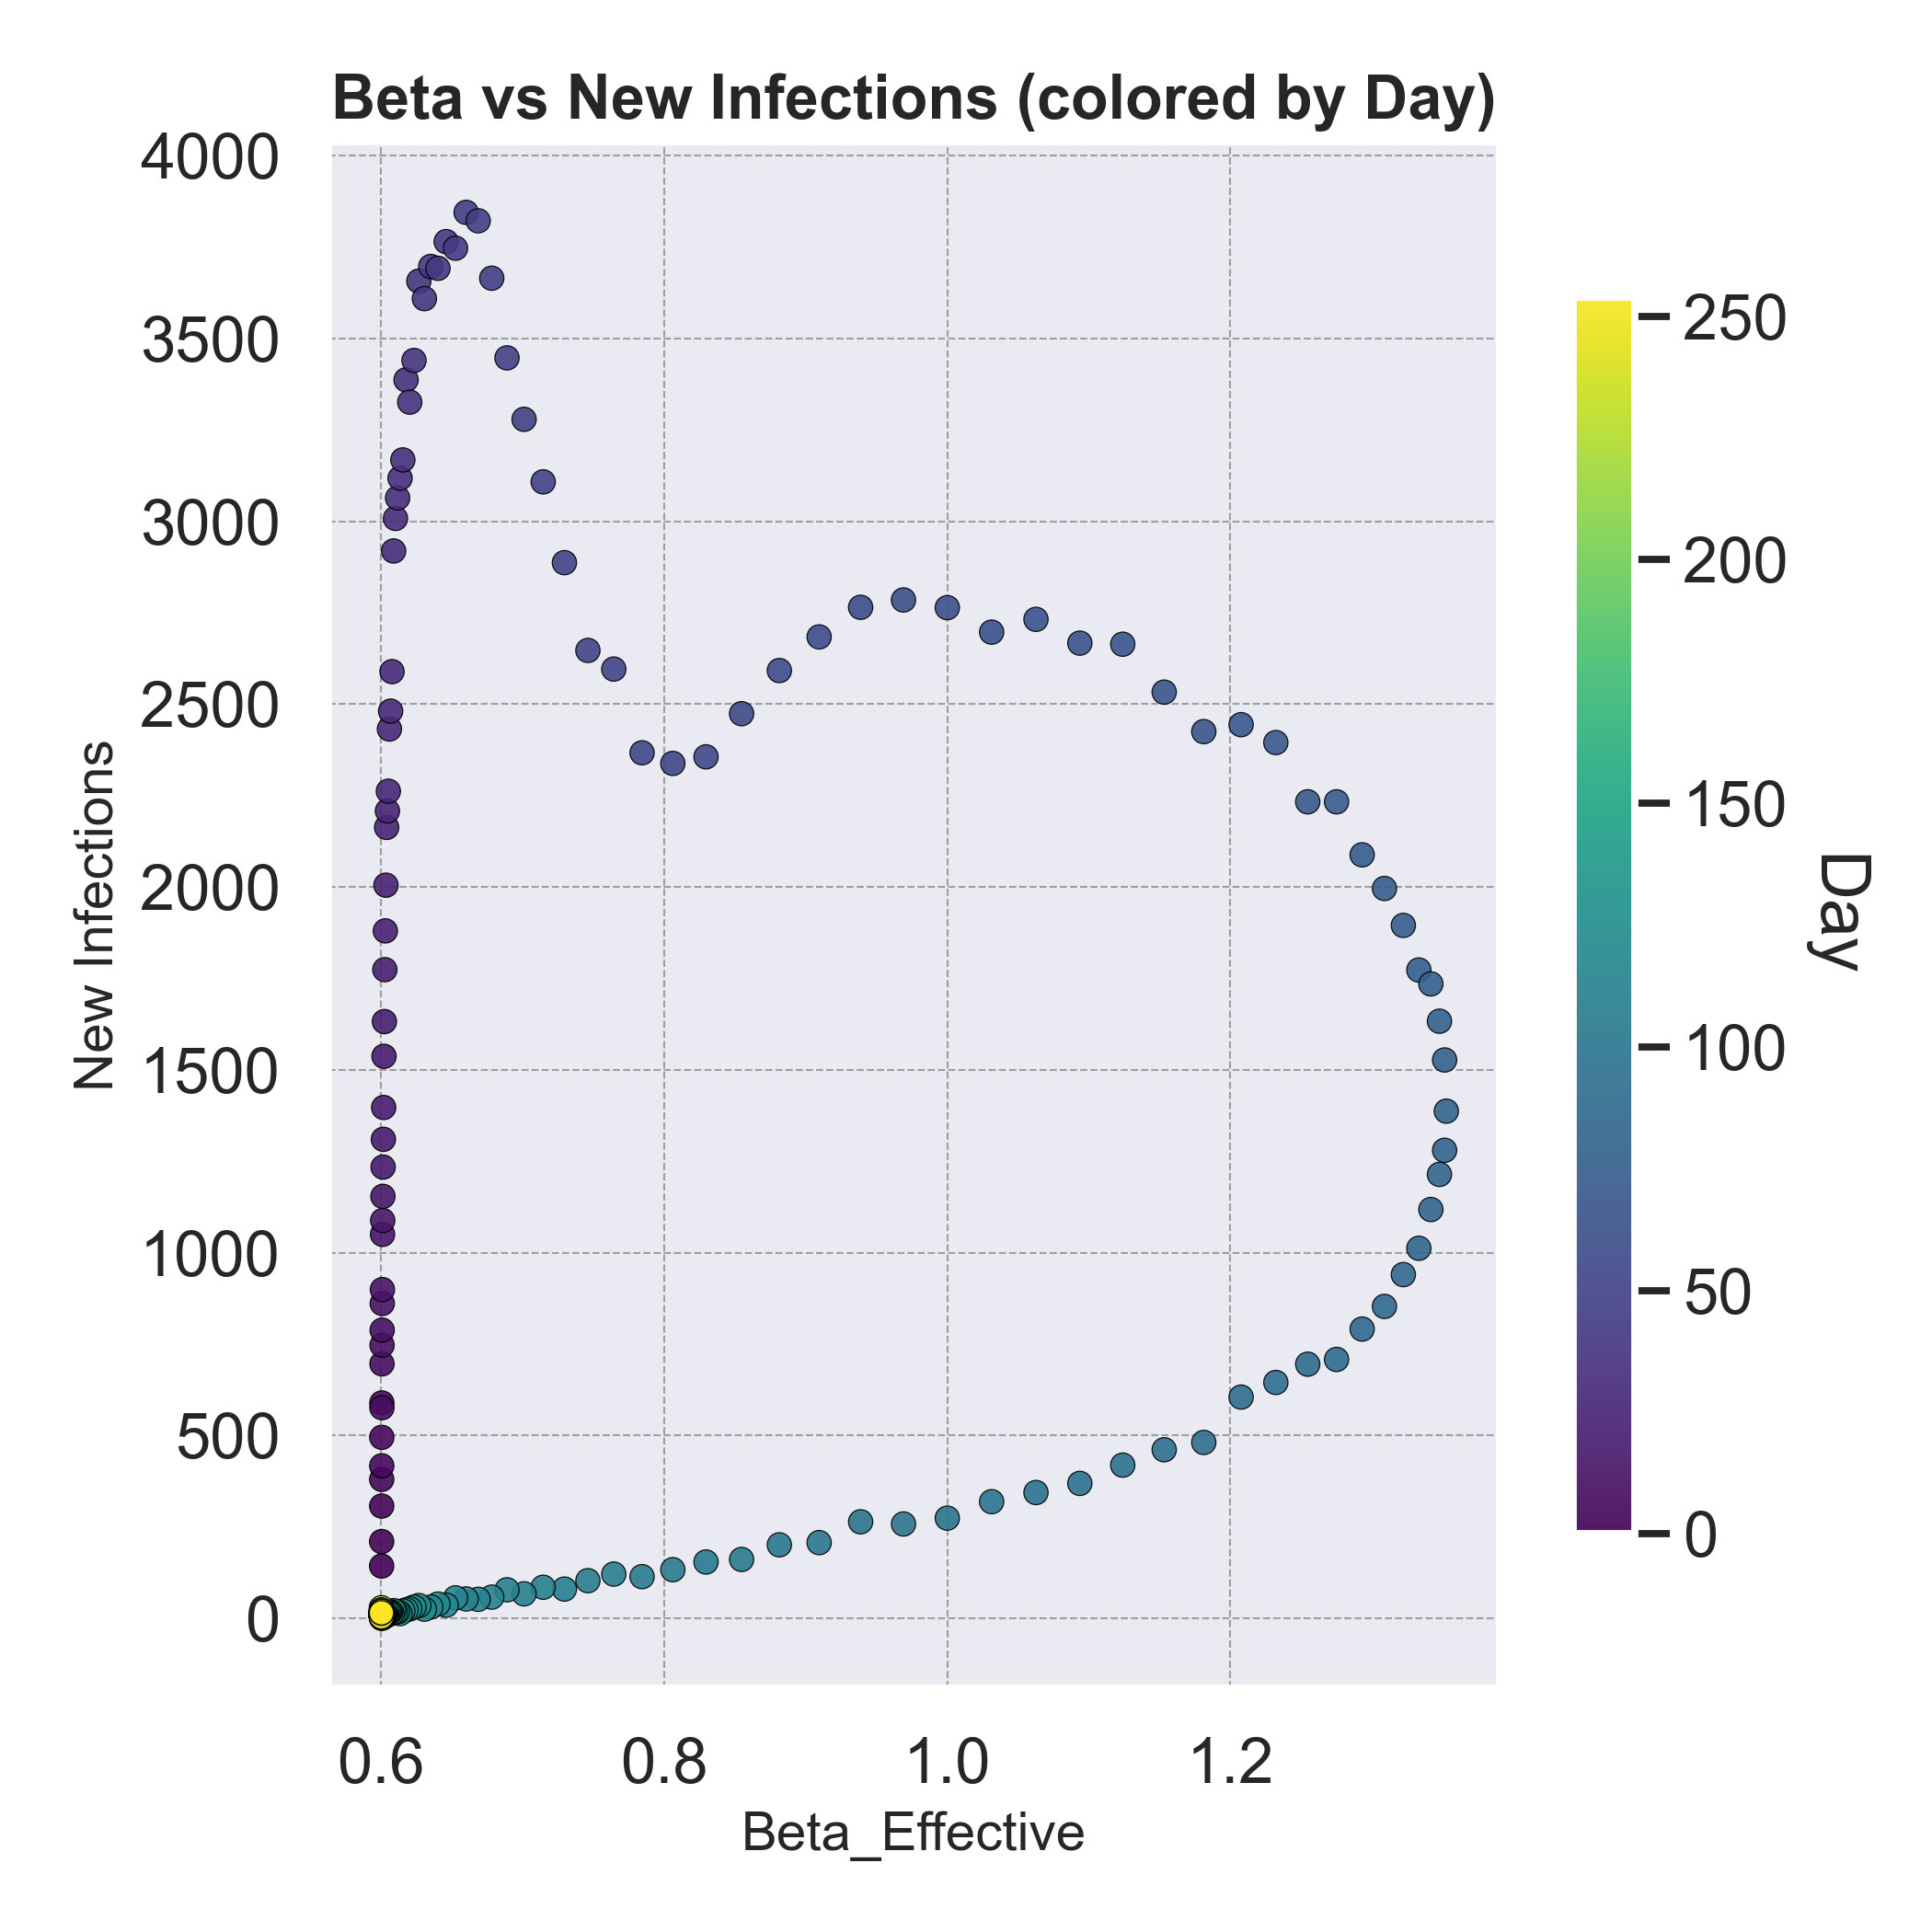
\includegraphics[width=\linewidth]{dil.png}
    \end{minipage}
    \hfill
    \begin{minipage}{0.49\linewidth}
        \flushright
        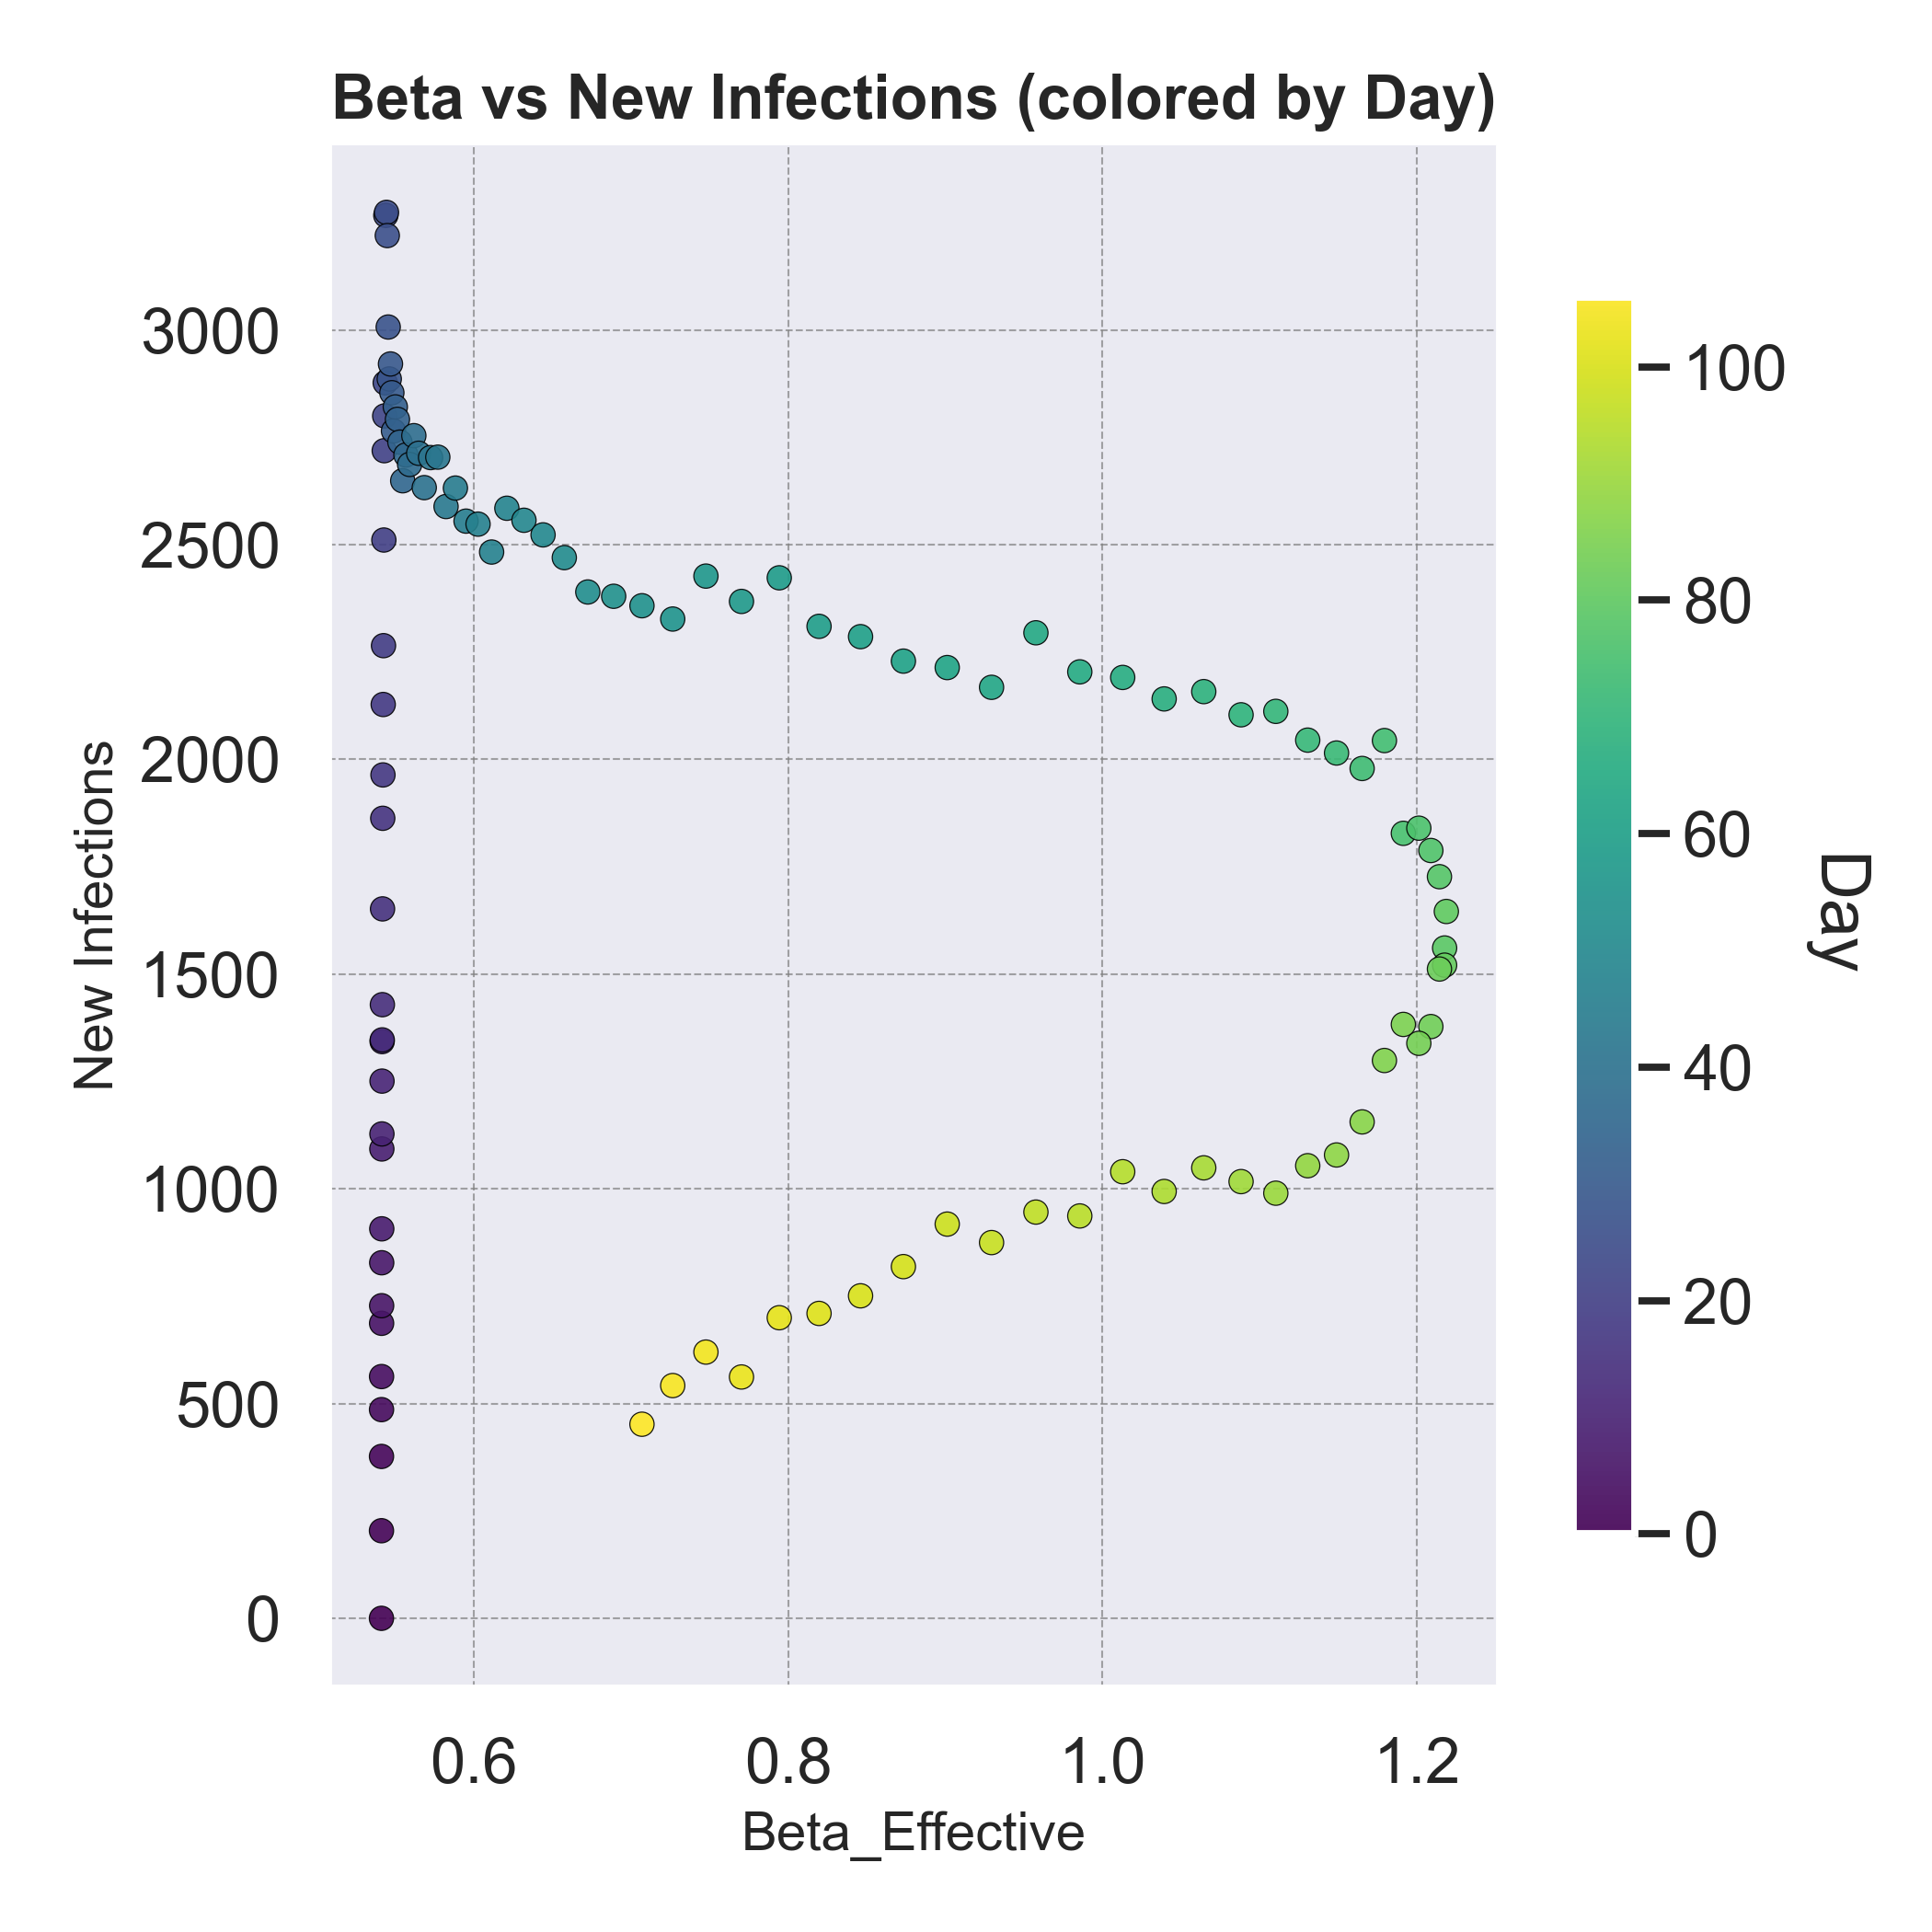
\includegraphics[width=\linewidth]{beta_vs_cases.png}
    \end{minipage}
    
    \caption{Beta vs. New Infections plot from a random batch}
    \label{fig:seir-side-by-side}
\end{figure}
\subsection{New Exposed vs New Recoveries}
This plot helps in epidemic growth detection. If New exposed > New Recoveries, the infection is spreading faster than its being cleared and if new exposed < new recoveries, it indicates decline of epidemic. \\
This plots often shows a crossover point where the two curves intersect each other. The first corssover signals the wave onset and the second crossover suggests wave resolution or success in interventions. \\
Reduced transmission is demonstrated by sharp dips in new exposed after a ploicy change for example lockdown and vaccination. If new recoveries continue to rise , it means that the healthcare system is still managing the previous cases, but future burden is dropping.
\begin{figure}[H]
    \begin{minipage}{0.49\linewidth}
        \flushleft
        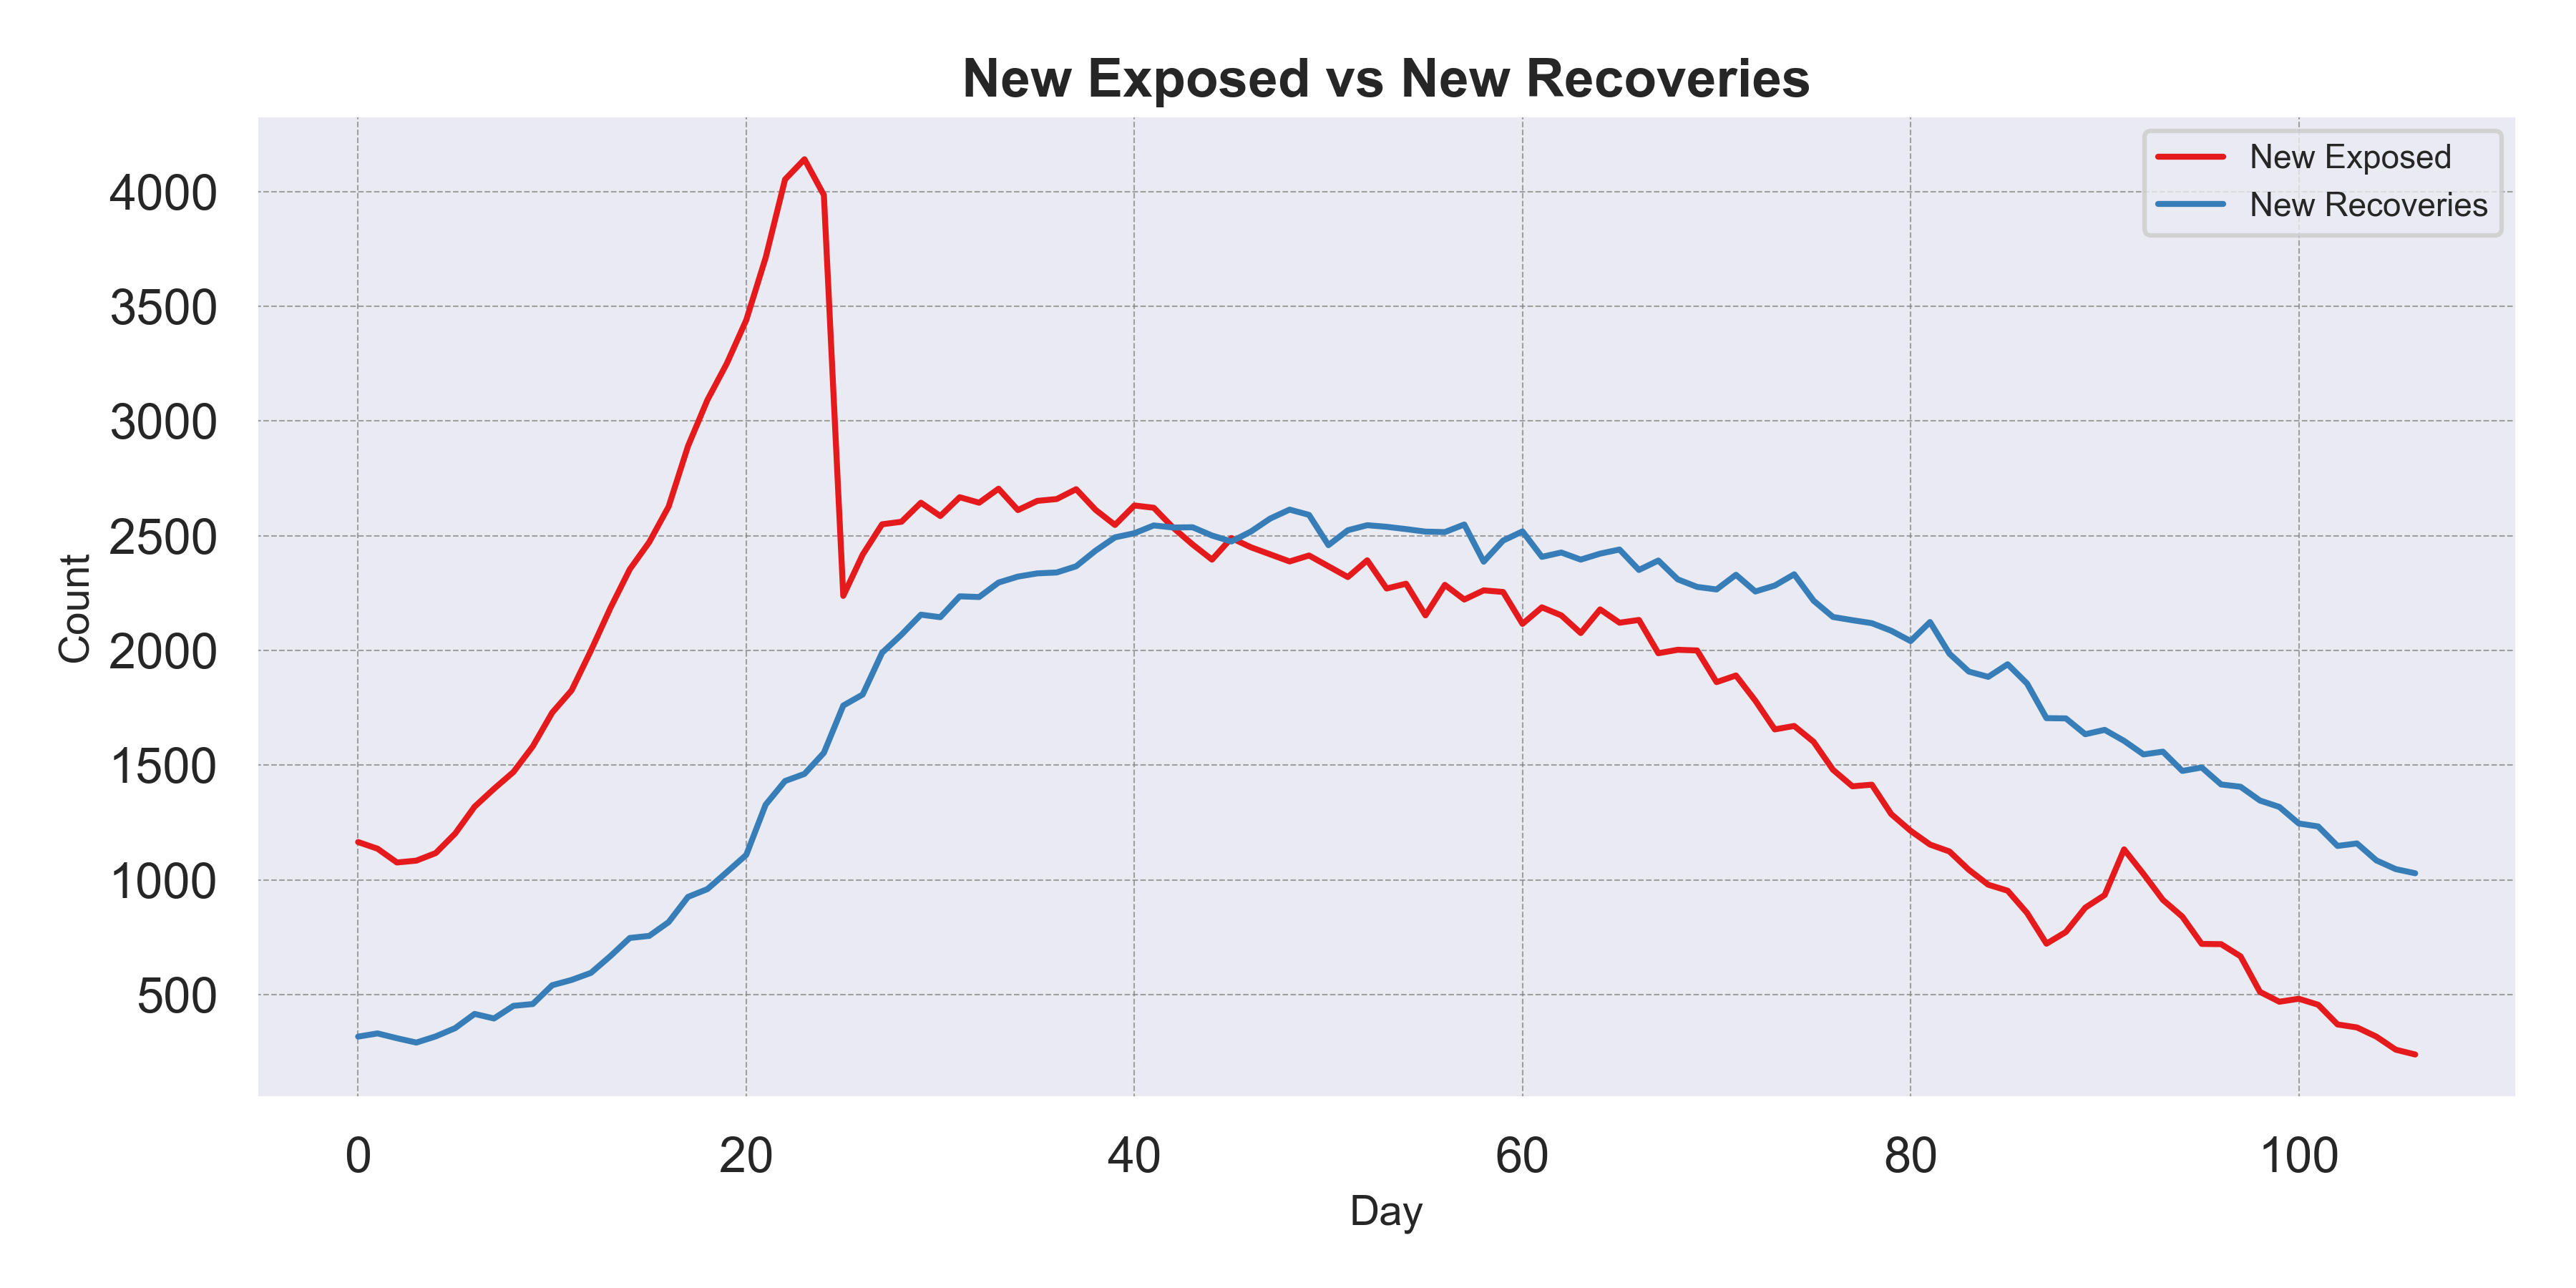
\includegraphics[width=\linewidth]{new_exposed_vs_recoveries.png}
    \end{minipage}
    \hfill
    \begin{minipage}{0.49\linewidth}
        \flushright
        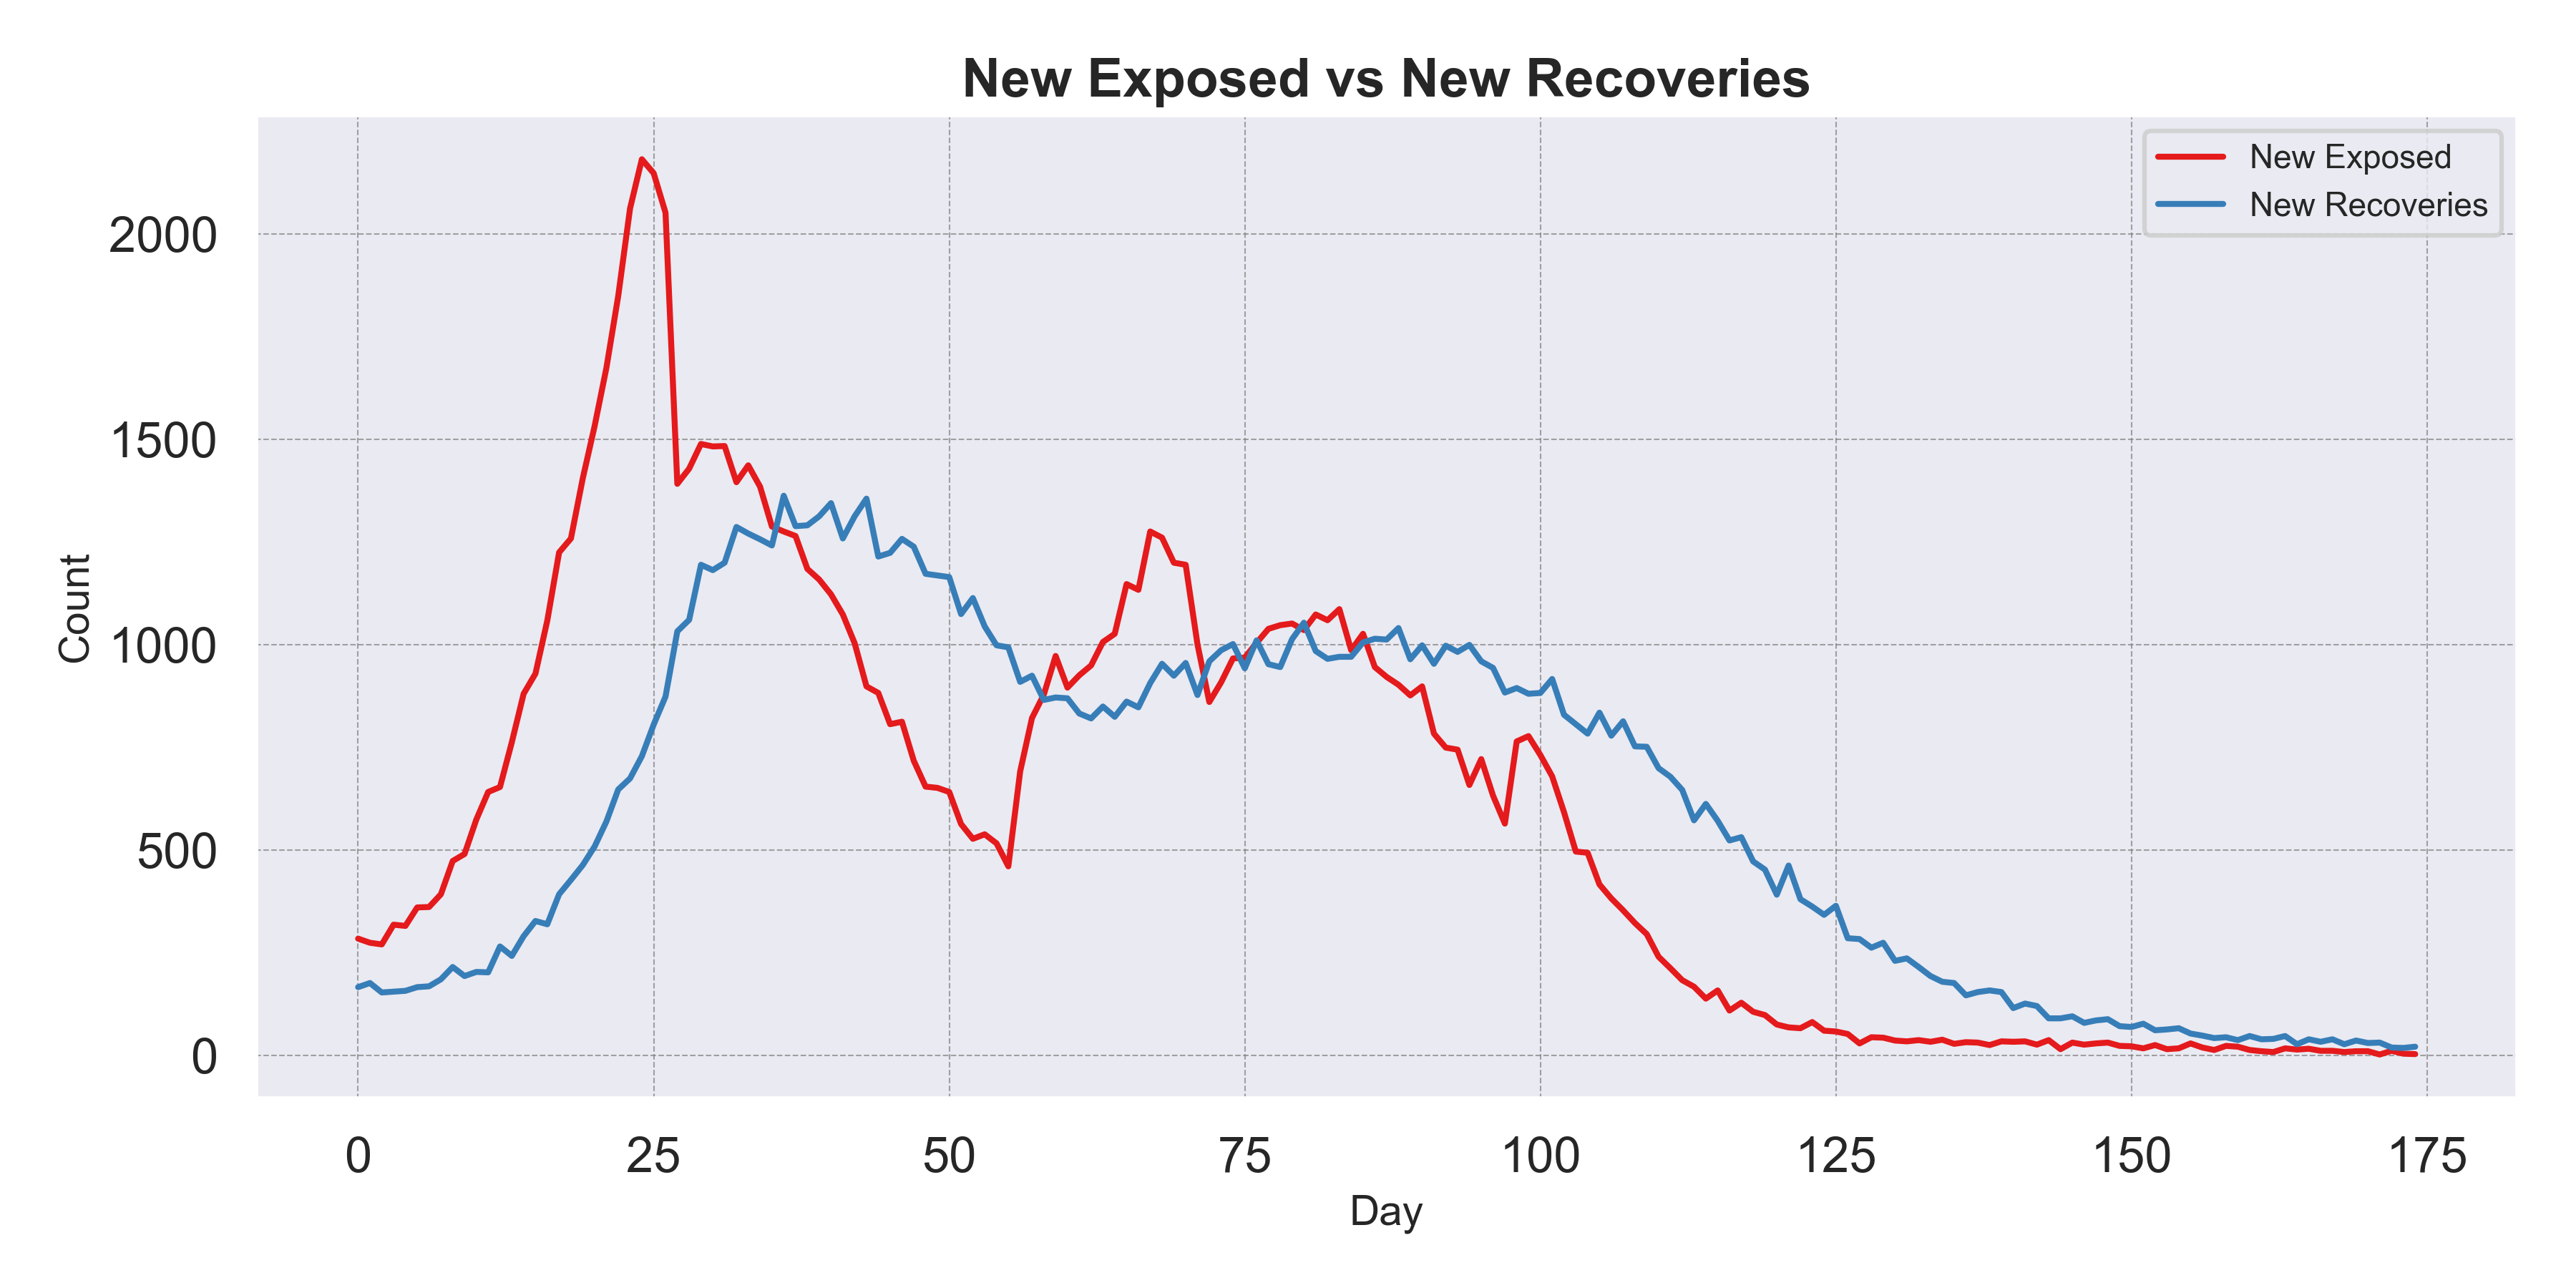
\includegraphics[width=\linewidth]{neee.png}
    \end{minipage}
    
    \caption{New Exposed vs New Recoveries plot from a random batch}
    \label{fig:seir-side-by-side}
\end{figure}
\subsection{Phase Diagrams}
Two types of phase diagrams are displayed, the I vs S diagram and the I vs R diagram, both colored by $\beta$ effective, in the I vs S phase plot, each point represents the system's state ona  given day, as the epidemic goes on, the system traces a trajectory through its space forming a loop or an arc, highliting the rise and fall of infections relating to the shrinking susceptible population.\\
The I vs R variant similarly tracks how infections transition into recoveris and it is particularly uselful for visualizing the cumulative impact of the epidemic. Unlike simpler plots, phase diagrams capture the entire system's evolution in a compact , geometric path , making them crucial for both theoretical exploration and practical modeling.
\begin{figure}[H]
    \begin{minipage}{0.49\linewidth}
        \flushleft
        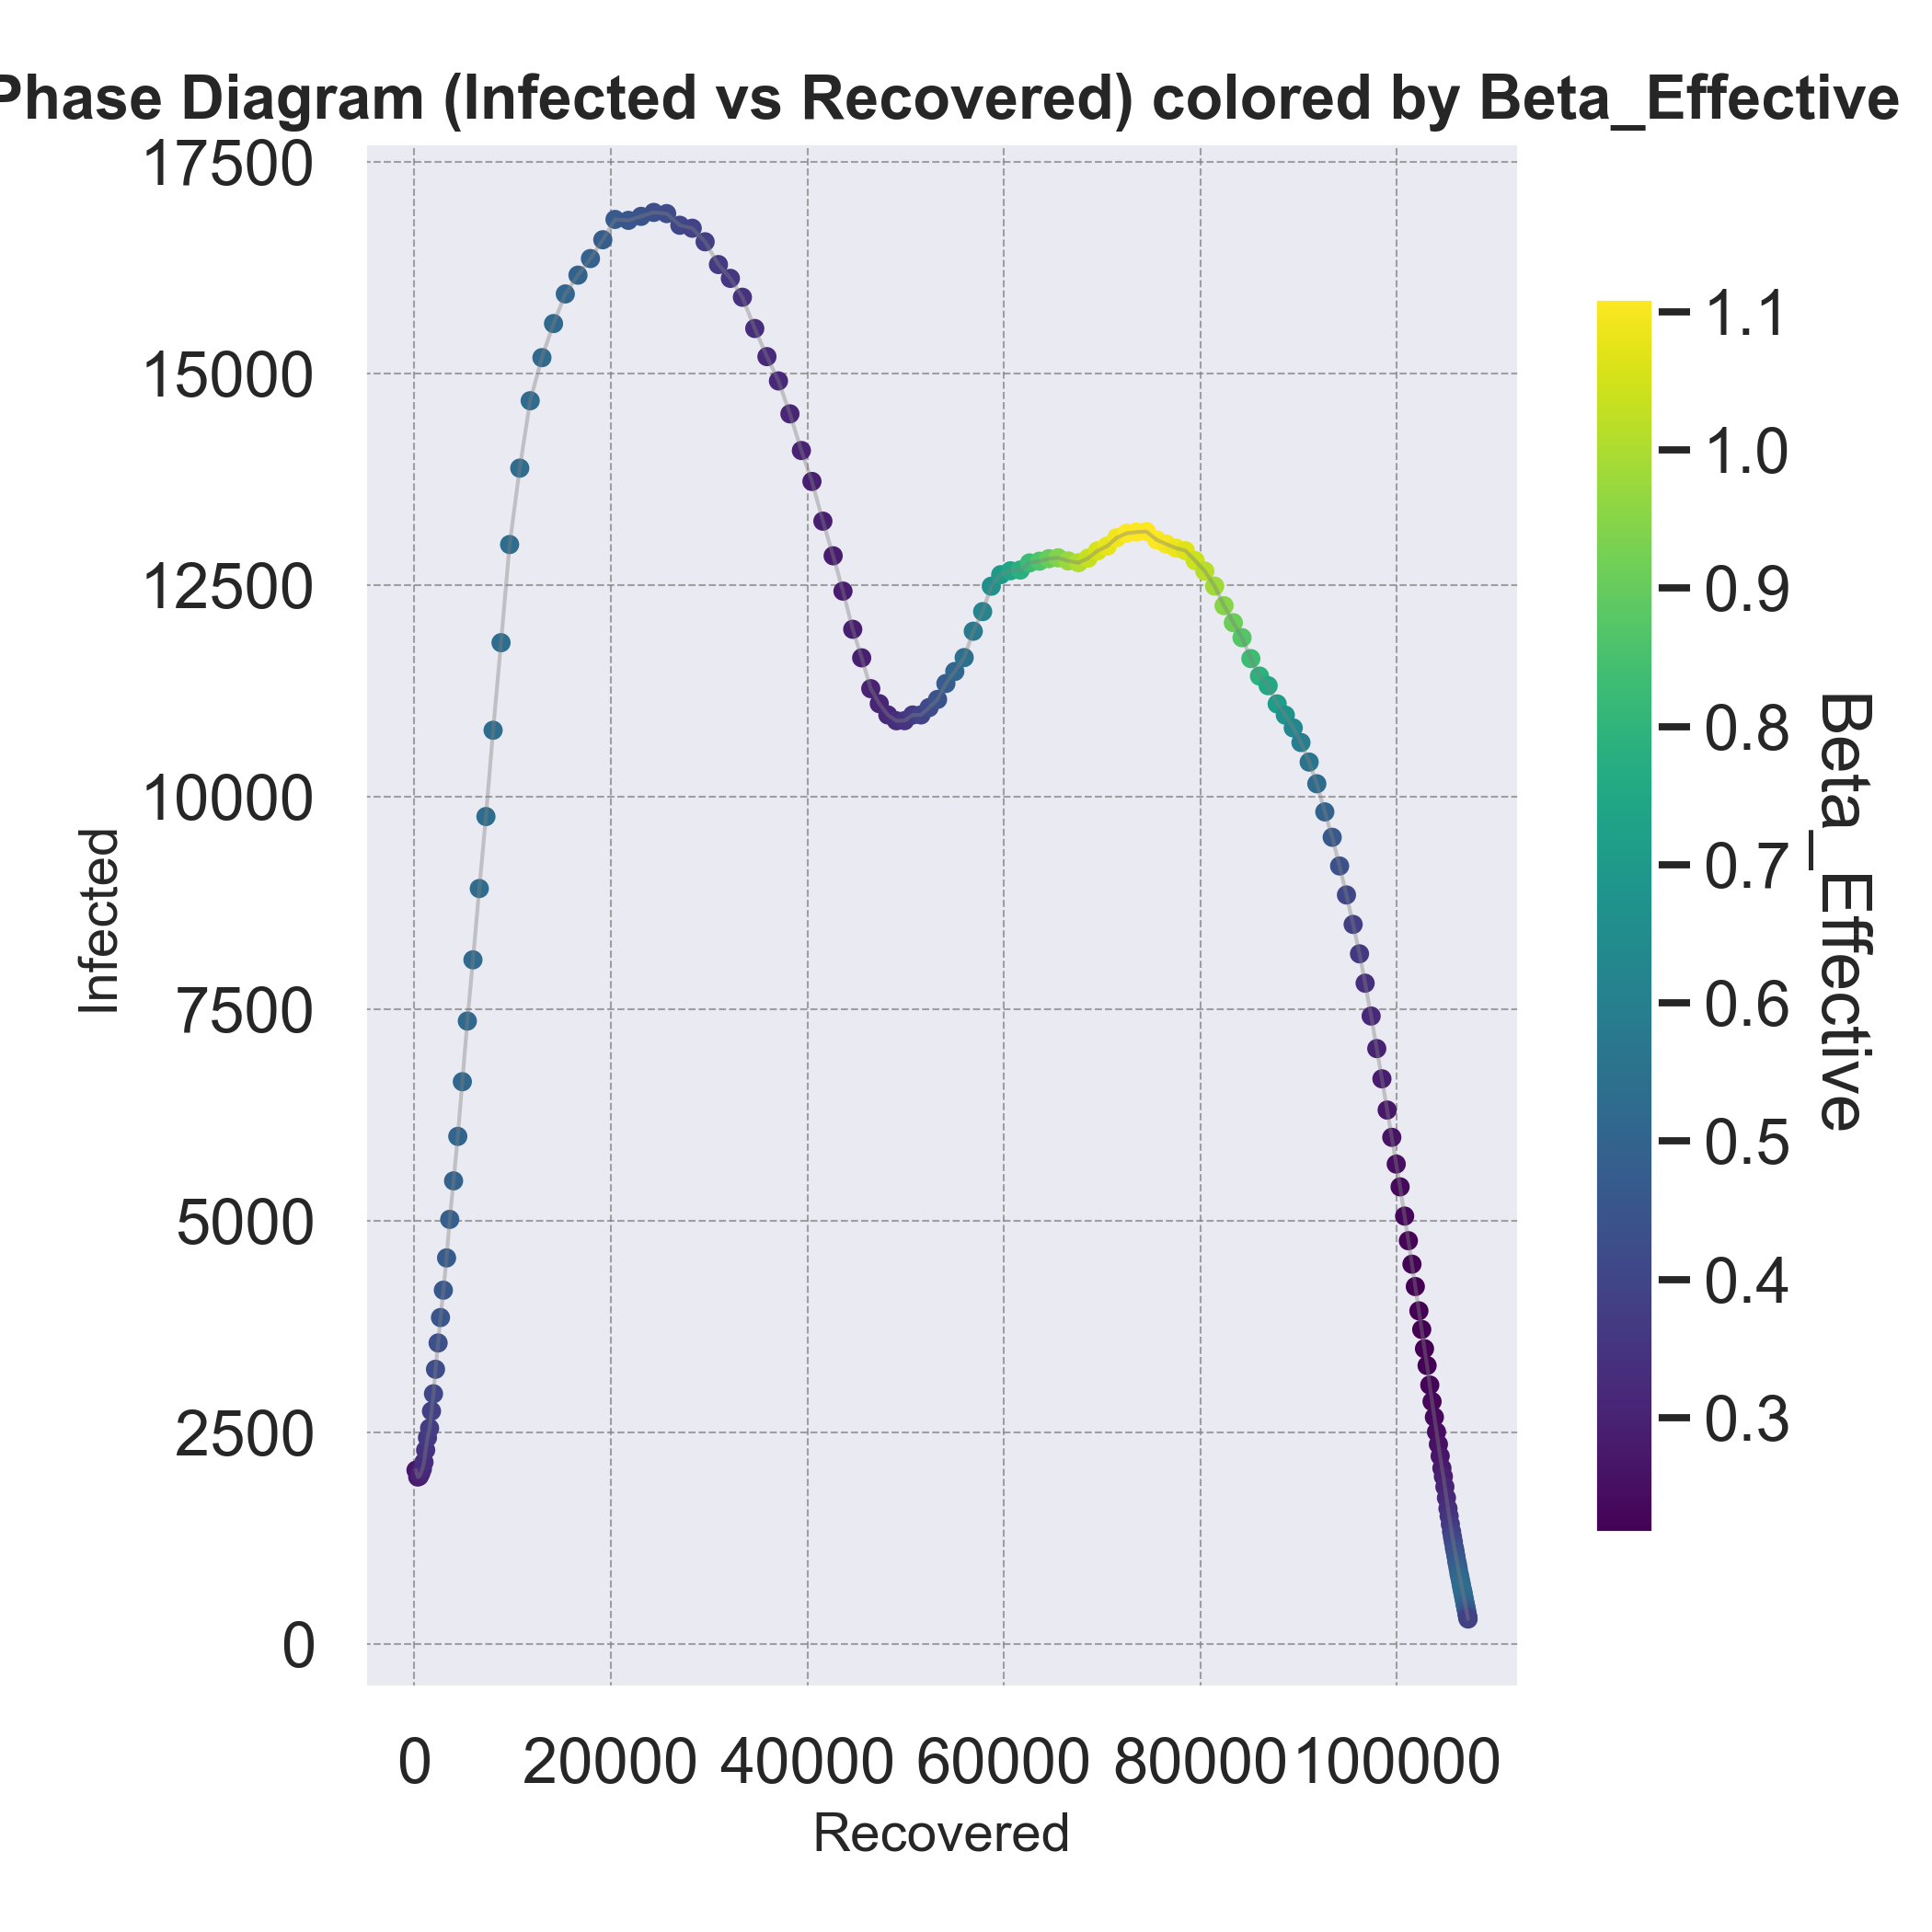
\includegraphics[width=\linewidth]{phase_I_vs_R_beta.png}
    \end{minipage}
    \hfill
    \begin{minipage}{0.49\linewidth}
        \flushright
        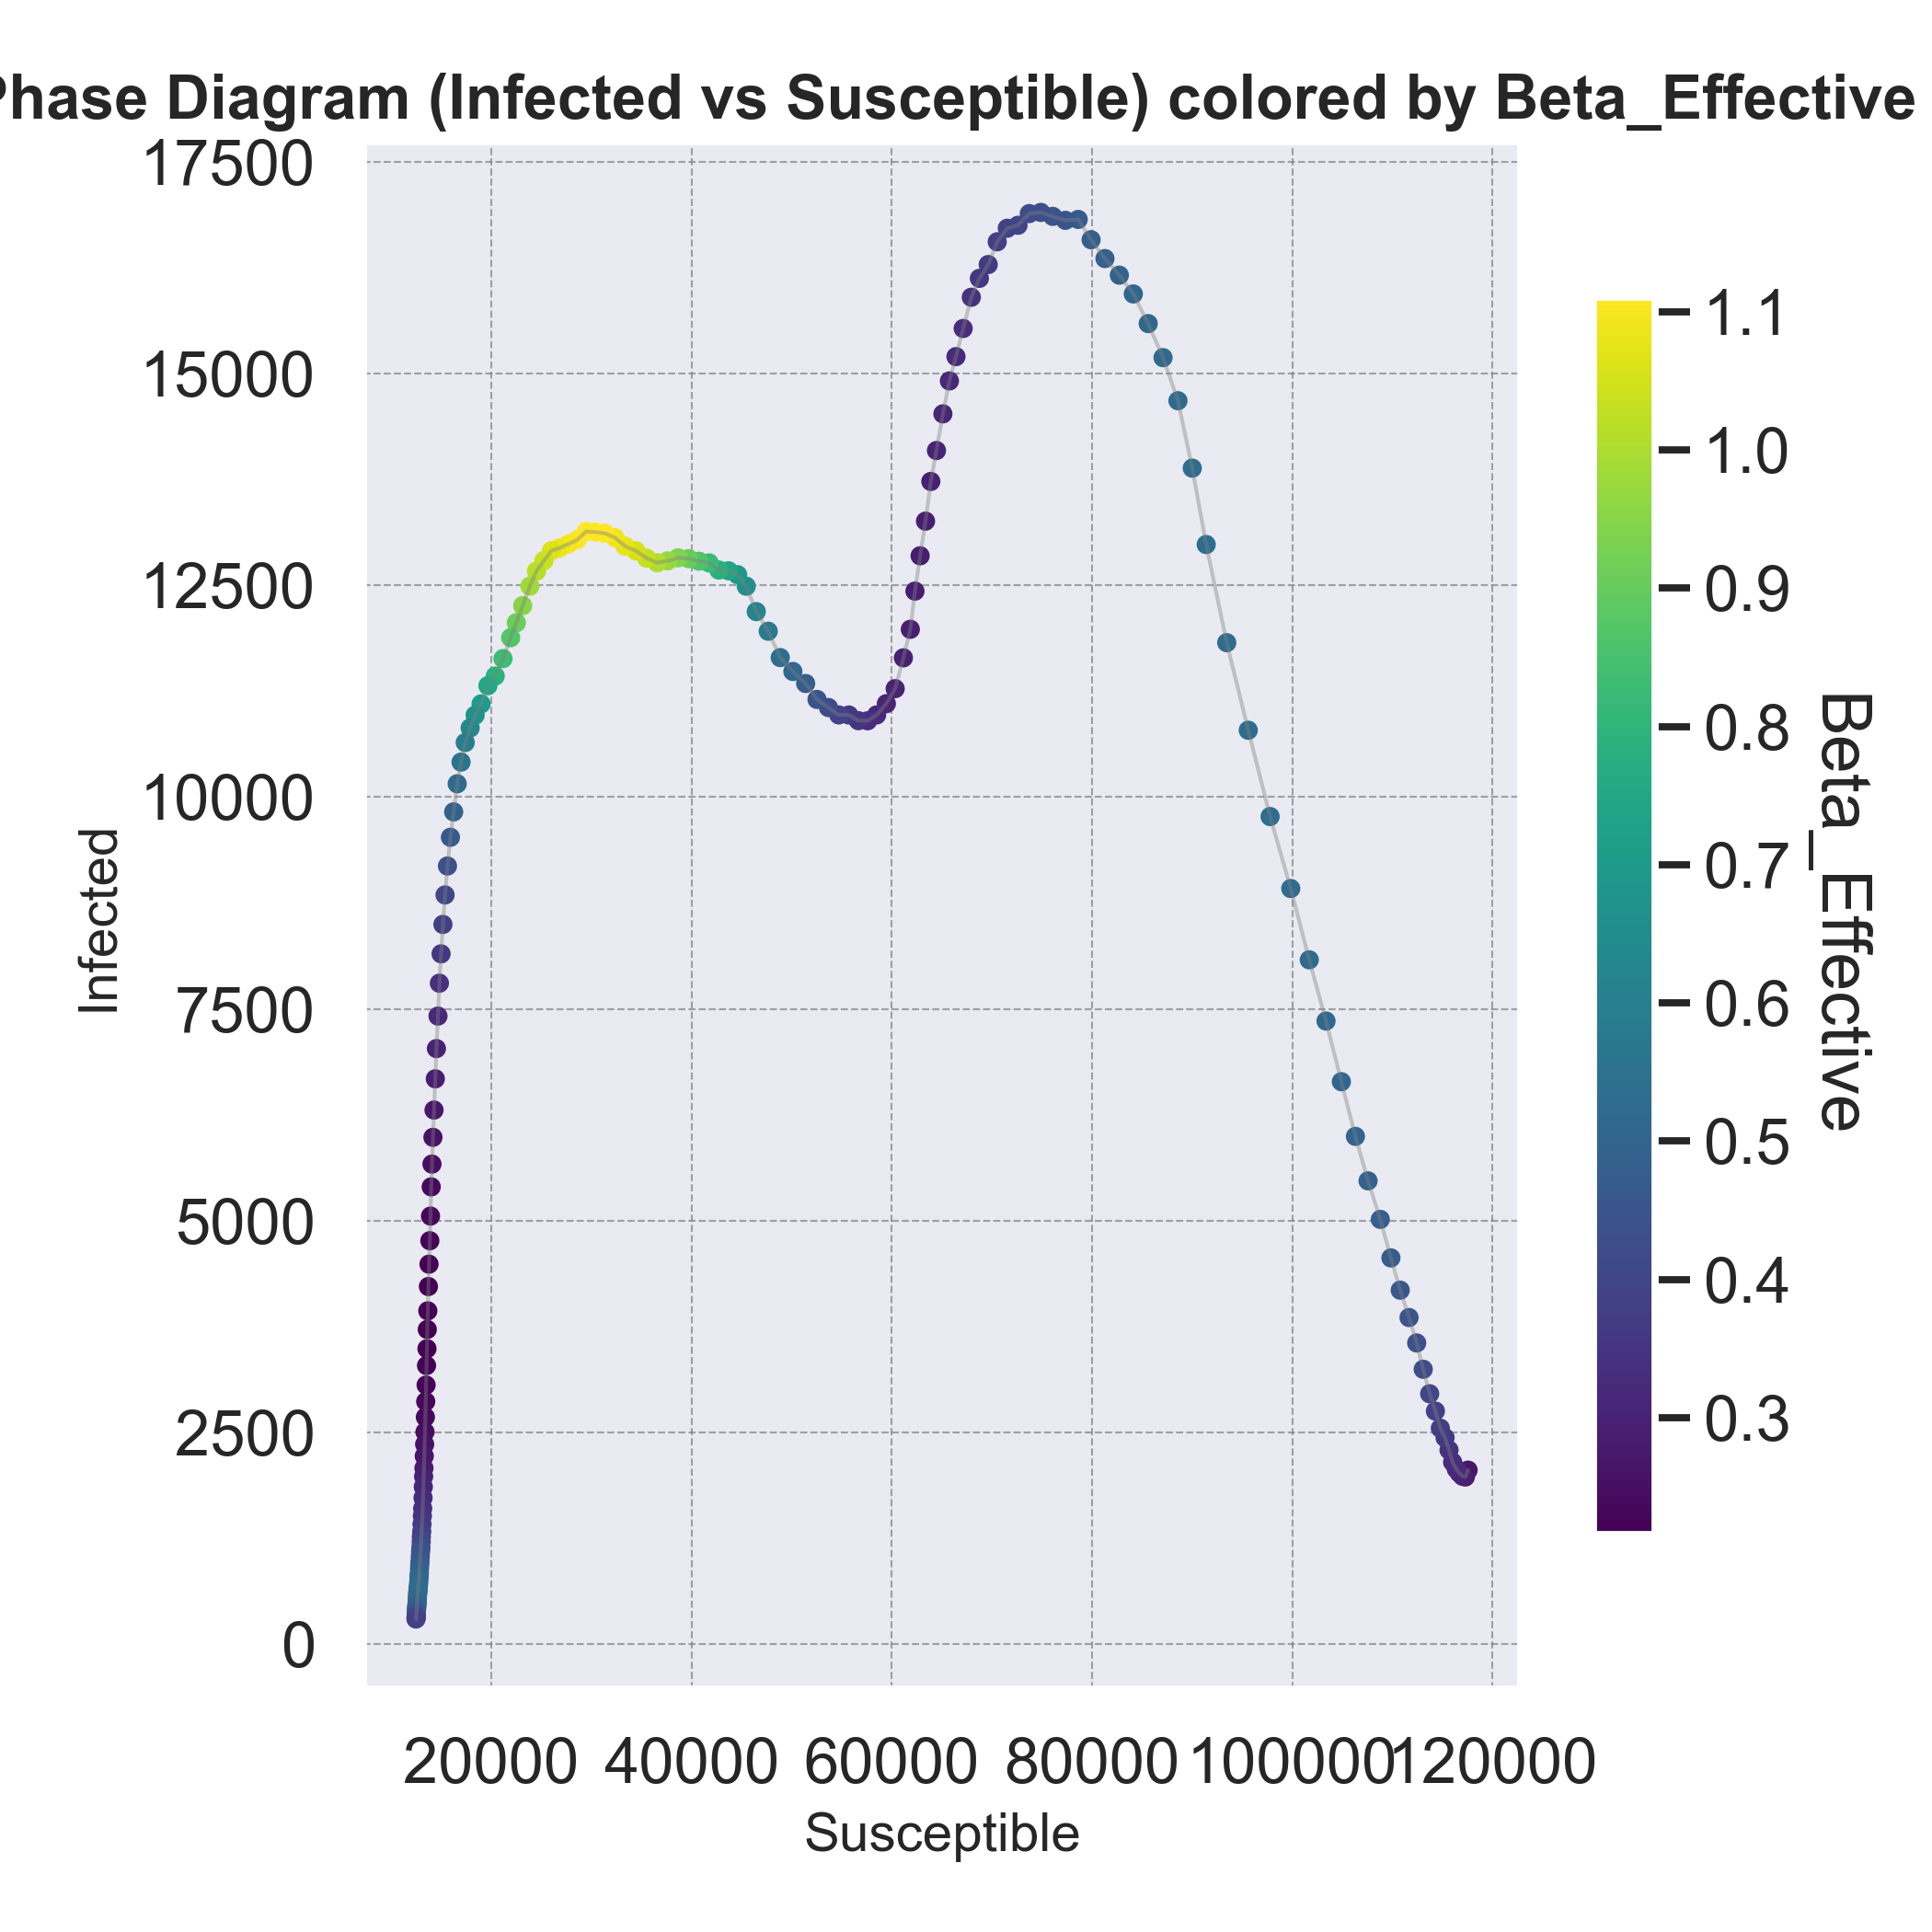
\includegraphics[width=\linewidth]{phase_I_vs_S_day.png}
    \end{minipage}
    
    \caption{Phase Diagrams from a random batch}
    \label{fig:seir-side-by-side}
\end{figure}
\subsection{Othe plots}
The \textbf{radial seasonality} plot uses a polar coordinate system to display cycles of seasons alongside infection levels, which makes it ideal for visualizing periodic disease where transmission rate is directly related to seasonality. The radial axis shows both seasonality strength and infection counts which allows user to correlate peaks in transmissiblity with actual outbreaks. \\
The \textbf{Reported vs Actual Infections} is a dual ine graph that compares reported cases with new infections which helps users to visualize under reporting, testing delays and observational noise. It is key for assessing the gap between observed date and true disease data , especialy in low testing regions and during surges. \\
\begin{figure}[H]
    \begin{minipage}{0.49\linewidth}
        \flushleft
        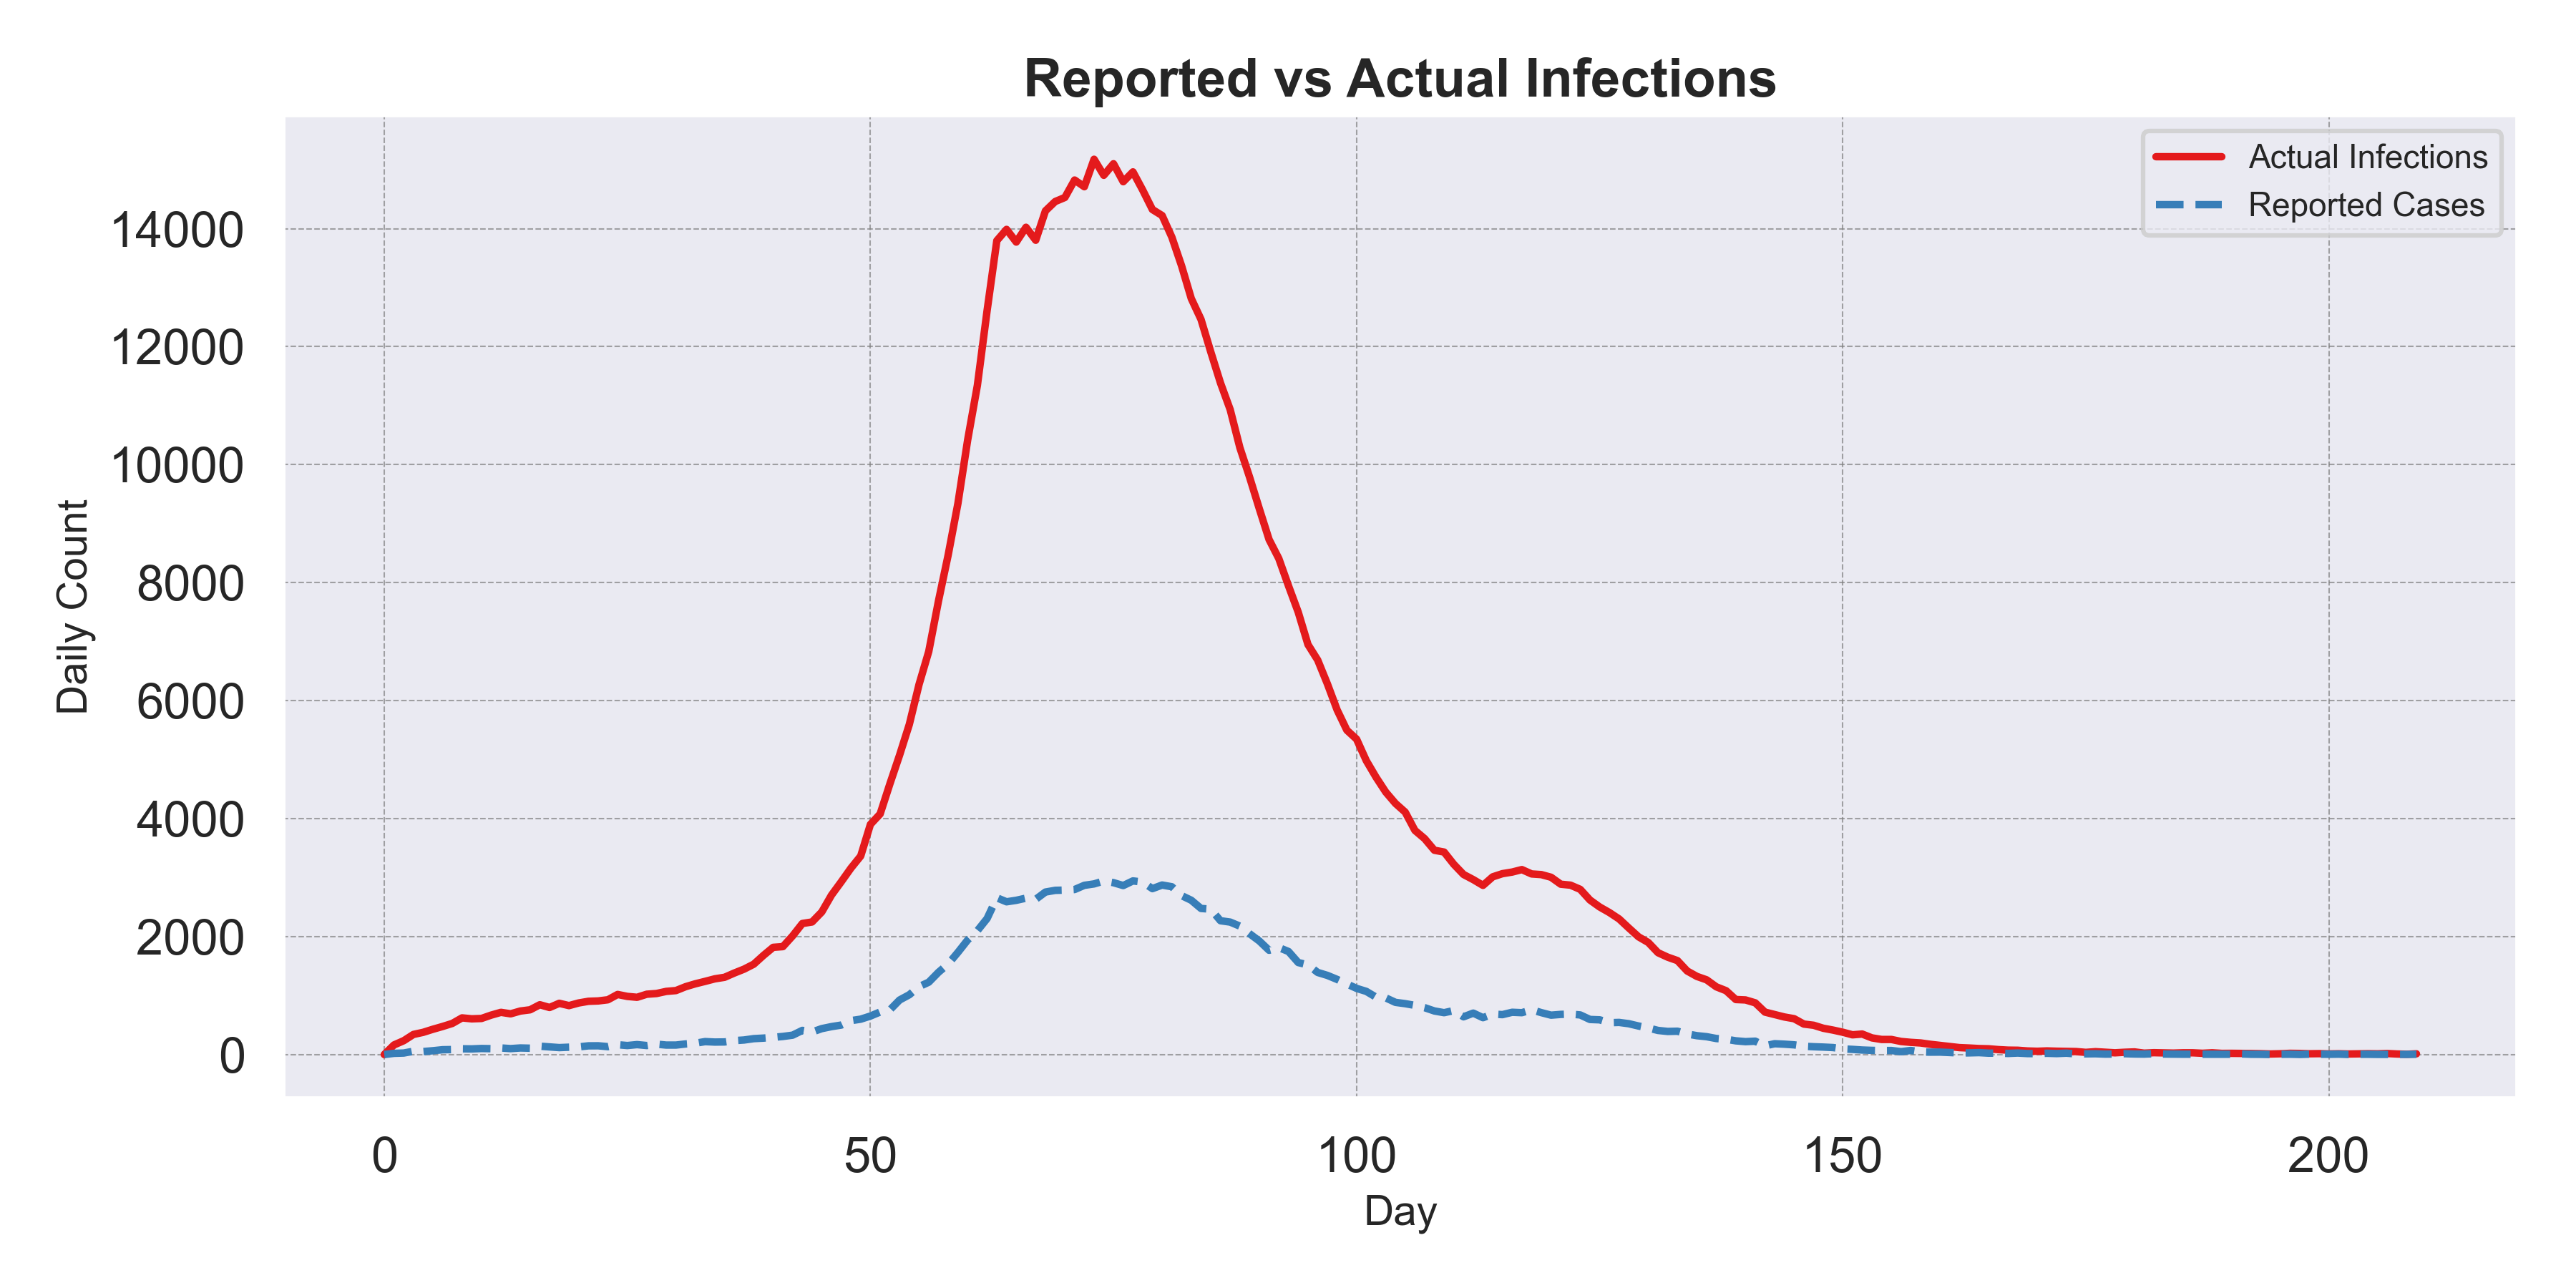
\includegraphics[width=\linewidth]{reported_vs_actual.png}
    \end{minipage}
    \hfill
    \begin{minipage}{0.49\linewidth}
        \flushright
        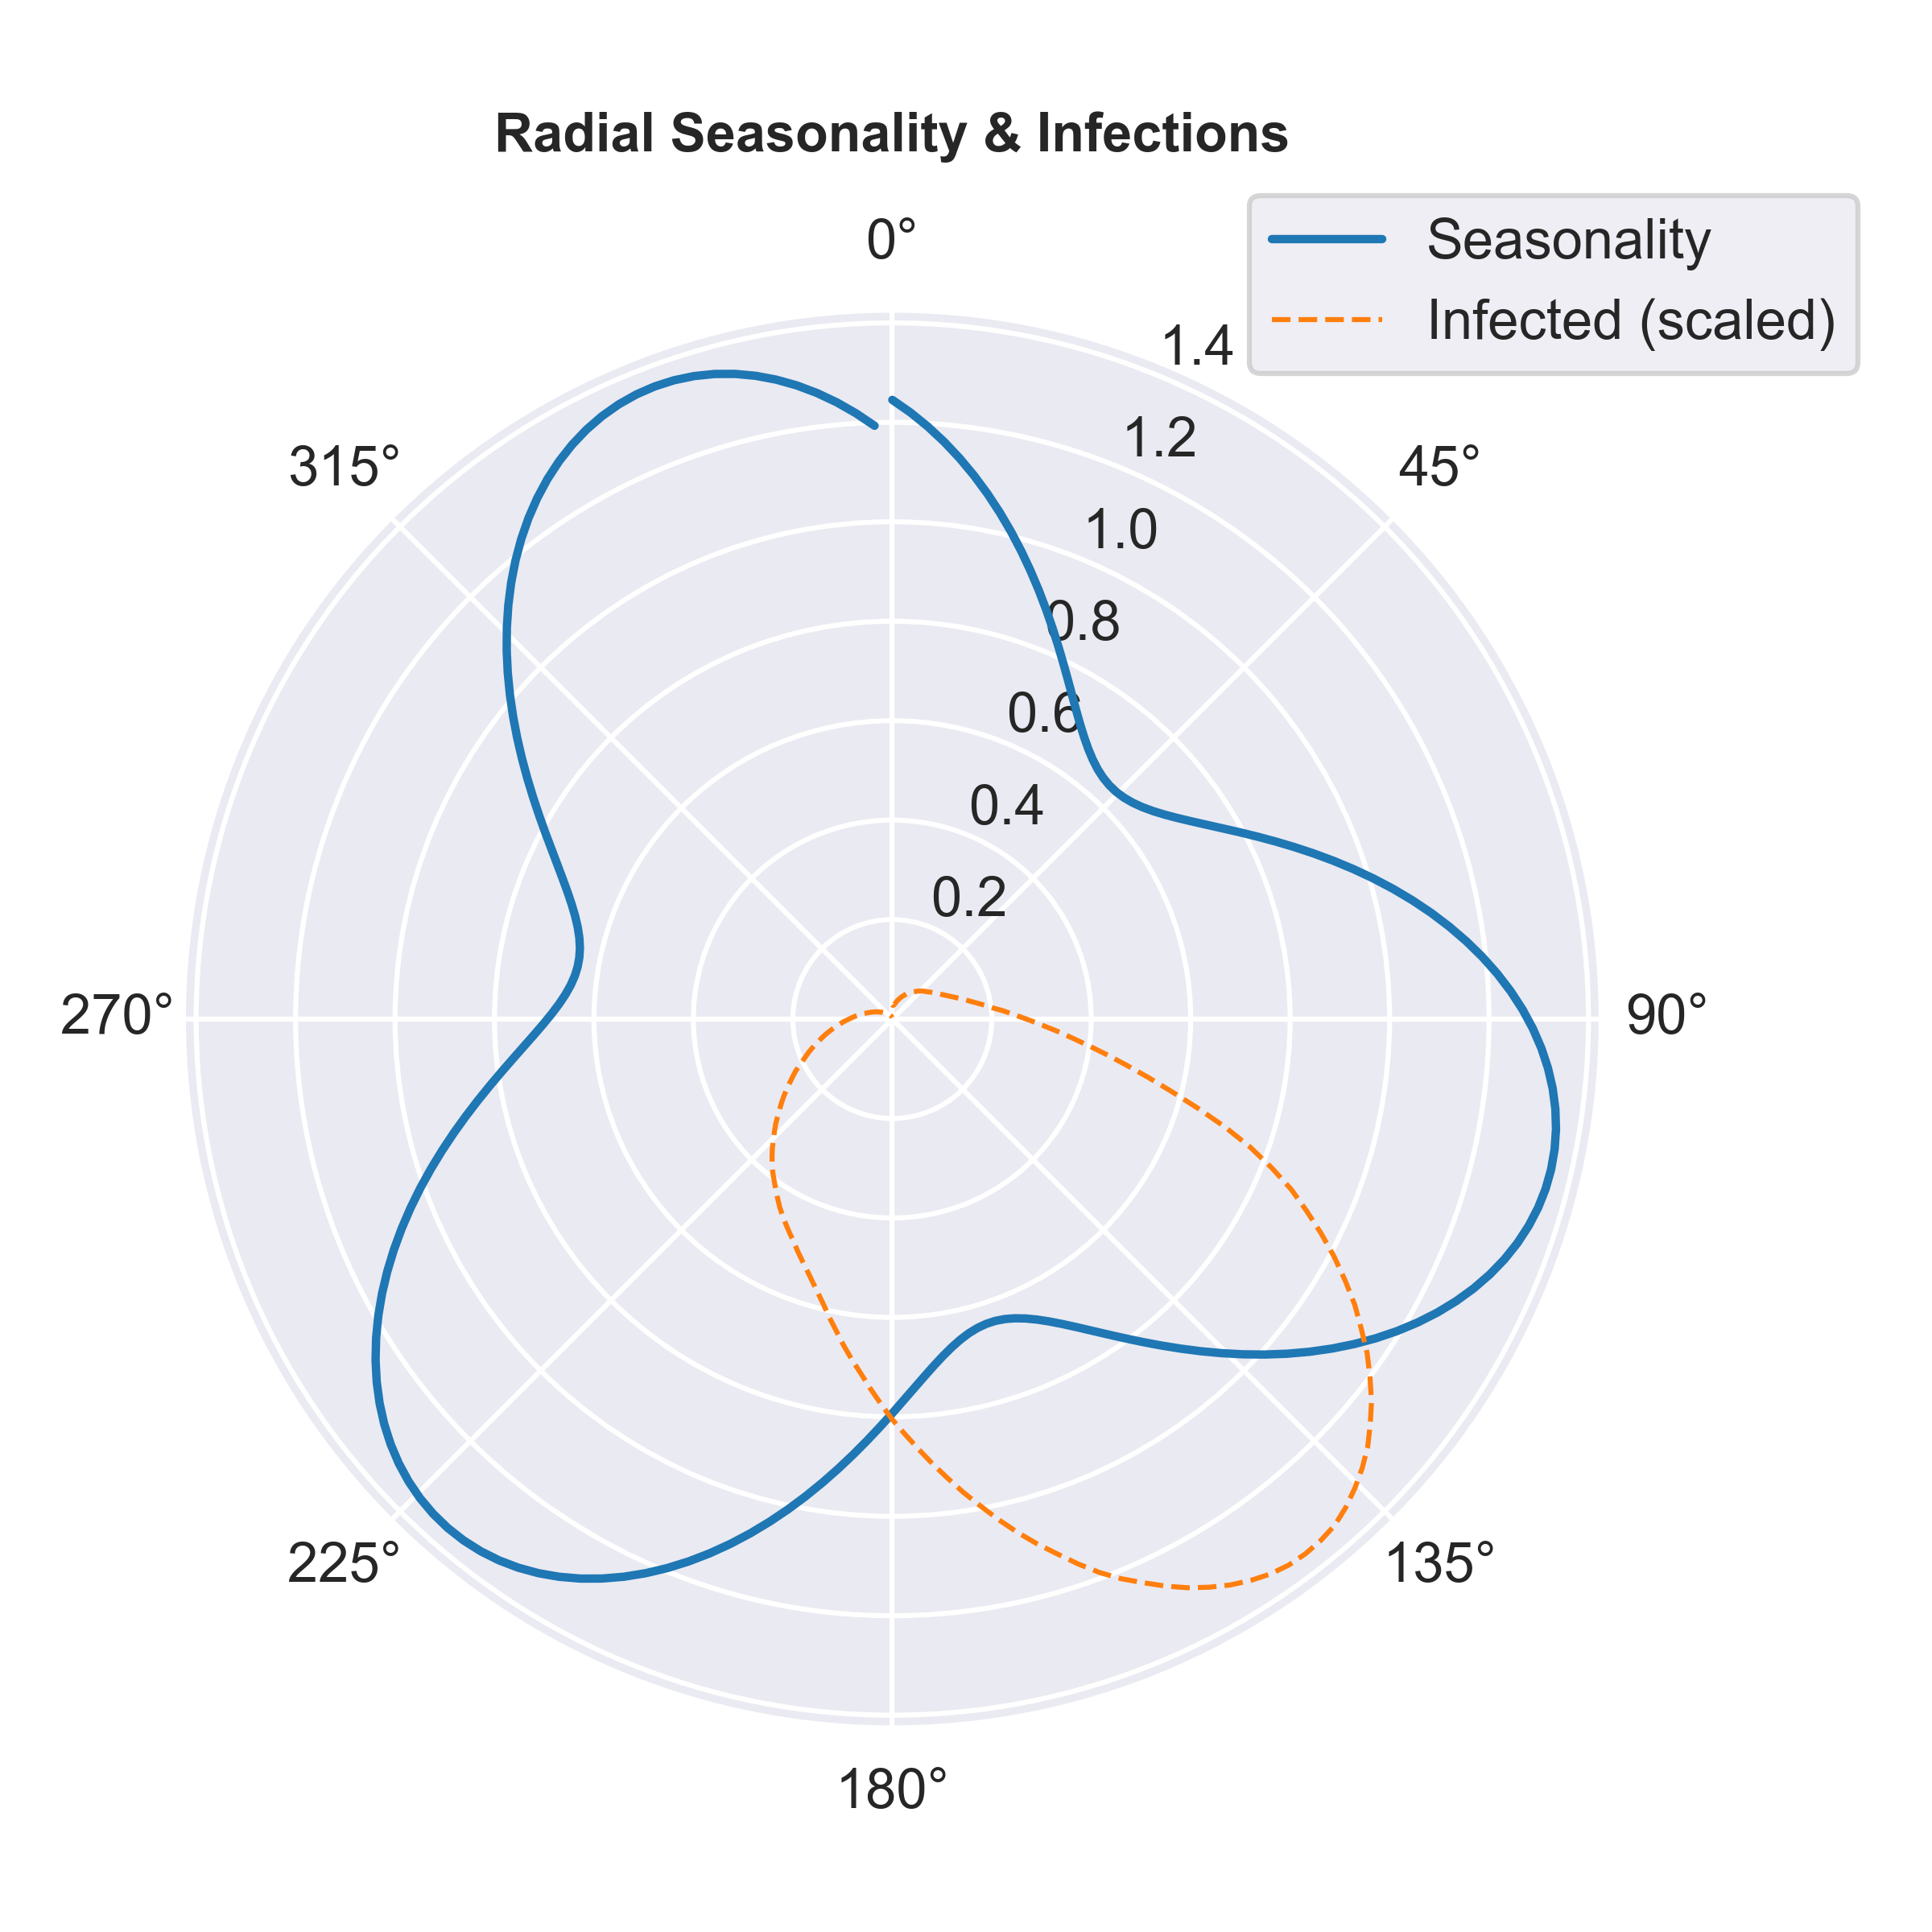
\includegraphics[width=\linewidth]{radial_seasonality.png}
    \end{minipage}
    
    \caption{}
    \label{fig:seir-side-by-side}
\end{figure}
\subsection{Comparison with real world date}
To evaluate the realism and validity of the synthethic data generated by our model, we have compared it with the actual COVID-19 daily reported cases in India (for the second wave).The data was taken from official website of WHO, it was first converted to BIGBOY format (it had only one column of reported cases) using a python script (available in GitHub), the comparison was run using another python script. We used scaling to match the range and resolution of synthethic outputs. The overall epidemic curve shape, peak structure and rise-fall dynamics have remained remarkably consistent across both datasets, despite manual feeding of parameters to BIGBOY1.2. We have done metric based comparisons between the two data below.\\
\begin{figure}[H]
    \centering
    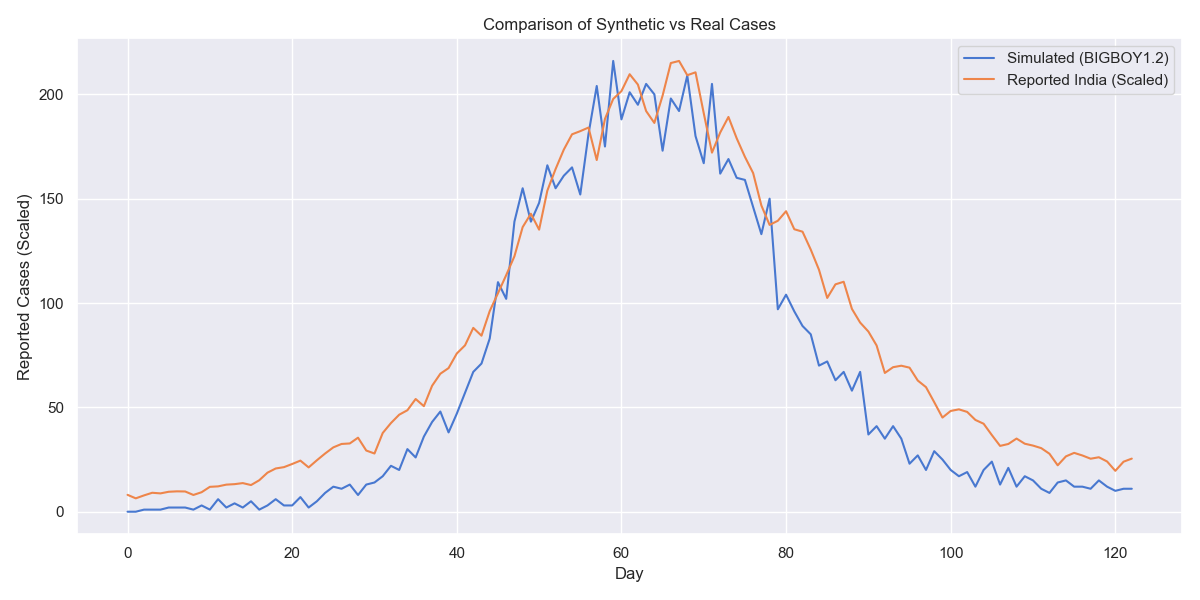
\includegraphics[width=1\linewidth]{ocn.png}
    \caption{COVID19 2nd wave compared to BIGBOY1.2}
    \label{fig:enter-label}
\end{figure}
\begin{table}[ht]
\centering

\arrayrulecolor{midgray}            % Border color
\setlength{\arrayrulewidth}{0.5pt}  % Border thickness

\rowcolors{1}{white}{lightgray}     % Zebra striping

\begin{tabular}{|>{\columncolor{lightgray}}l|c|c|}
\hline
\textbf{Metric} & \textbf{Real Data} & \textbf{BIGBOY1.2 Simulated} \\
\hline
Basic Reproduction Number ($R_0$) & 1.29 & 1.16 \\
Epidemic Duration (Days) & 53 to 71 & 51 to 70 \\
Peak Infection Days (Top 3) & 67, 68, 59 & 59, 68, 67 \\
\hline

\end{tabular}

\arrayrulecolor{black}  % Reset color for future tables
\caption{Comparison of COVID-19 vs BIGBOY1.2}
\end{table}
\subsection{Sources of Deviation}
The shape of the waves depict promising overlap, there are still scopes of improvement, these deviations are not unexcepted and can be attributed to several factor like \textbf{real world data complexity} , publicly available data suffers from factors like inconsistent testing , region specific anomalies. Extracting granular data would improve graph alignment more. Another factor is \textbf{parameter calibration}, BIGBOY1.2 uses manually selected parameters, which is good for understanding curves and real world factors but when it comes to mimicking real world curves, automated hyperparameter tuning ( like Bayesian optimization) would match real epidemics more precisely. These changes would be incorporated in the next version of BIGBOY.\\
These minor discrepancies between the simulated and observed curves do not stem out from model inaccuracies, rather it is the inherent stochasticity and undetermined variables that play in the real world outbreaks. In fact, real world epidemics are so chaotic that even the same virus would behave differently if replayed in the same conditions. 

\section{Future Work (BIGBOY1.3)}
BIGBOY1.2 provides a great platform for generating synthethic disease outbreak data but its development is not completed yet. We have planned to include several powerful extensions for future versions, the roadmap includes the following improvements : 
\subsection{Enhanced Visualizations}
We aim to include an animate mode as --animate X (X being different animated visuals) to make outbreak visualizations more dynamic and interactive. This mode would include layered epidemic progression, animated transmission waves and geospatial spread mapping. We would also be integrating agent based and grid based simulations to complement the compartmental SEIR model. This will allow us to see a individual level perspective,  mobility and stochasticity, it would help in capturing phenomena like superspreading and localized interventions.
\subsection{Disease mode}
A new interface would be implemented in the CLI, which would allow the use to select from pre-configured templates for diseases like COVID-19, measles, influenza and more. Each of these templates would include pre loaded parameters, allowing faster and disease specific scenario generation and modelling. The mode could be accessed as --disease X (X being the disease template). We would also expand on the intervention parameters and healthcare system constraints would also be implemented. A better multiwave structure would also be configured.
\subsection{Automated Hyperparameter Tuning}
BIGBOY1.3 will feature automated hyperparameter tuning using techniques such as Bayesian Optimization and grid search, which will calibrate parameters directly from real datasets, which could be used in scenarios where limited amount of data is available for a particular disease and BIGBOY1.3 could be used to generated unlimited disease like data using AHT. 
\subsection{Country mode}
BIGBOY1.3 will also feature a country mode where user could select from all the countries and a set of calibrated parameters would be applied to them. These parameters would include population, crowding, literacy (corresponding to mask adherence and vaccinations), country specific behaviors, population pyraminds (dividing population into categories) and seasonality profies. \\
Let us understand capabilites of BIGBOY1.3 using an example
\begin{center}
\tcbox[
  colback=blue!5,
  colframe=black!50,
  boxrule=0.5pt,
  arc=0mm,
  boxsep=5pt
]{% The content goes in the braces
 --disease EBOLA --country INDIA --state HARYANA --animate GRID
}
\end{center}
This would simulate disease outbreak of EBOLA in Haryana, India. Though EBOLA has never hit Haryana, but the model contains both the profiles for EBOLA and Haryana and will flawlessly simulate and generate datasets for Ebola Outbreak in Haryana.
\subsection{Ramen1}
We are working on several SVR, SIR, SEIR and FDE based models and their hybrids to make SOUP S-1 (SVR-SIR) , CRUM1 (SVR-SEIR), Broth-N (Naive baseline based SVR) and SVR-FDE models, further this model soup would be merged into a high fidelity ensemble system named Ramen1 , which would combine best of all approaches using weighted voting and time series. 
\section{Open Source and Contributions}
BIGBOY1.2 is open source and could be used for unrestricted academic and non-commercial use. The complete codebase along with sample datasets from BIGBOY1, BIGBOY1.1 and BIGBOY1.2 are publicly available on GitHub. \\
A short demo video demonstrating how to run BIGBOY1.2 on your local machine is available on Youtube. \\
We encourage students and researchers to use BIGBOY1.2 to understand and simulate epidemic curves and we are open to contributors who would like to be a part of BIGBOY1.3 and further improvements. For contribution purposes, mail here. \\
Ramen1 is the bigger project which required generation of a synthethic dataset, that's how BIGBOY1 came into being. Ramen1 used many sub models to predict disease outbreak, it switches between various model depending on the phase of the outbreak (ensemble model). It is still work in progress,  if anyone wants to contribute in Ramen1 , send a mail here. \\
\subsection{Acknowledgements: } The author (Raunak Narwal) would like to thank \textbf{Prof. Syed Abbas} for this internship opportunity which led to this project.\\
The author would also like to thank \textbf{Rishu Narwal}, Phd candidate at IIT Delhi, for  helping out with research literature, structure of the research paper and providing a computational support.\\
Special thanks to \textbf{Chirag Verma}, third year undergraduate studetn at IISER Mohali, for his theoretical insights and discussions in the area of epidemic outbreak modeling.

\bibliographystyle{apalike} 
\bibliography{references}  

\vspace{4mm}
\begin{center}
\textit{\large ``Thanks''} \\
\end{center}
\end{document}


